% !TEX root = documento.tex
%% ========================================================================== %%
%% Projeto Integrado de Extensão - Karaokê Apache (Apache Gru Rock Bar)       %%
%% Estruturado no Template ABNTeX2 / ABNTEX-IFPI (Pronto para Overleaf)       %%
%% ========================================================================== %%

%% Classe do documento (definida aqui para que este seja o único arquivo raiz do projeto)
\documentclass[
	12pt,				% Fonte: 12pt
	oneside,			% Impressão: oneside = 1 face, twoside = 2 faces (frente-e-verso)
	a4paper,			% Tamanho do Papel: A4
	chapter=TITLE,		% Todos os capítulos devem ficar em caixa alta
	section=TITLE,		% Todas as seções devem ficar em caixa alta
	english,			% Adiciona Idioma para Hifenização: Inglês
	brazil				% Adiciona Idioma para Hifenização: Português do Brasil (principal)
]{abntex2}				% Utilizar ABNTeX2

%% Preâmbulo (configurações, pacotes e tudo mais)
% !TEX root = ../documento.tex
%% Preâmbulo LaTeX: Define classes e características do documento
%% A classe do documento (\documentclass) fica em documento.tex

%% Tipografia (Arial / Helvetica por padrão)
%% Tipografia / Fontes
%% Latin Modern (fonte padrão do LaTeX / exemplo-proj-extens-c.pdf, com suporte completo a acentuação)
\usepackage{lmodern}

%% Outras opções (comentadas):
%\usepackage{mathptmx}
%\usepackage{helvet} \renewcommand{\familydefault}{\sfdefault}


%% Pacotes usados pelo documento
\usepackage{courier}
\usepackage[T1]{fontenc}
\usepackage{textcomp}
\usepackage[utf8]{inputenc}
\usepackage{indentfirst}
\usepackage{nomencl}
\usepackage{color}
\usepackage{graphicx}
\usepackage{float}
\usepackage{needspace}
\usepackage{microtype}
\usepackage{lastpage}
\usepackage{booktabs}
\usepackage{multirow, array, tabularx}
\usepackage{titlesec}
\usepackage[table,xcdraw]{xcolor}
\usepackage[brazilian,hyperpageref]{backref}
\usepackage{simplecd}
\usepackage[final]{pdfpages}
\usepackage{listings}
\usepackage{amsmath, amssymb}

%% Adiciona as alterações do ABNTeX-IFPI
\usepackage{abntex-ifpi/abntex-ifpi}
\usepackage{abntex-ifpi/tikz-uml}

%% Configuração de listagens de código-fonte com suporte a UTF-8
\definecolor{codebg}{RGB}{246,248,250}
\definecolor{codeframe}{RGB}{208,215,222}
\definecolor{codecomment}{RGB}{87,96,106}
\definecolor{codekeyword}{RGB}{5,80,174}
\definecolor{codestring}{RGB}{10,48,105}

\lstset{
  backgroundcolor=\color{codebg},
  basicstyle=\ttfamily\footnotesize,
  breakatwhitespace=false,
  breaklines=true,
  captionpos=t,
  commentstyle=\color{codecomment}\itshape,
  frame=single,
  rulecolor=\color{codeframe},
  keepspaces=true,
  keywordstyle=\color{codekeyword}\bfseries,
  numbers=left,
  numbersep=8pt,
  numberstyle=\tiny\color{codecomment},
  showspaces=false,
  showstringspaces=false,
  showtabs=false,
  stringstyle=\color{codestring},
  tabsize=2,
  literate={á}{{\'a}}1 {é}{{\'e}}1 {í}{{\'i}}1 {ó}{{\'o}}1 {ú}{{\'u}}1
           {Á}{{\'A}}1 {É}{{\'E}}1 {Í}{{\'I}}1 {Ó}{{\'O}}1 {Ú}{{\'U}}1
           {à}{{\`a}}1 {ã}{{\~a}}1 {õ}{{\~o}}1 {ç}{{\c{c}}}1 {Ç}{{\c{C}}}1
           {ê}{{\^e}}1 {ô}{{\^o}}1 {â}{{\^a}}1
}

%% Comandos auxiliares para Apêndices e Anexos
\newcommand{\apendiceitem}[2]{\chapter{#1}\label{#2}}
\newcommand{\anexoitem}[2]{\chapter{#1}\label{#2}}

%% Metadados, citações, cores e espaçamentos
%% Configurações dos metadados do PDF
\makeatletter
\hypersetup{
  pdftitle={\@title}, 
  pdfauthor={\@author},
  pdfsubject={Projeto Integrado de Extensão - IFSP Campus São Paulo},
  pdfcreator={LaTeX, abntex2, {abnTeX\-ifpi}},
  pdfkeywords={Sistema web}{Karaokê}{Gerenciamento de fila}{Electron}{React}{Projeto de extensão},
  colorlinks=true,
  linkcolor=cor-link,
  citecolor=cor-link,
  filecolor=cor-link,
  urlcolor=cor-link,
  bookmarksdepth=4
}
\makeatother

%% Metadados do trabalho
\titulo{Karaokê Apache: Sistema Integrado de Gerenciamento de Fila, Pedidos Musicais e Reprodução para Bar de Karaokê}
\autor{João Pedro Rodrigues \\ Josee Hoshi Vellani Bellintani \\ Leonardo Gutierrez Mamani \\ Luiz Eduardo Barbosa Silveira \\ Murillo Andrade Assis \\ Yasmin Bonfim de Moraes}
\nomedocurso{Tecnologia em Análise e Desenvolvimento de Sistemas}
\local{São Paulo, SP}
\preambulo{Relatório Técnico apresentado como exigência parcial para avaliação na disciplina de Projeto Integrado de Extensão do Curso de Tecnologia em Análise e Desenvolvimento de Sistemas do Instituto Federal de Educação, Ciência e Tecnologia de São Paulo, Campus São Paulo.}
\orientador{Prof. M\textsuperscript{e}. Marcelo Tavares de Santana}
\tipotrabalho{Relatório Técnico}
\data{2026}
\instituicao{INSTITUTO FEDERAL DE EDUCAÇÃO, CIÊNCIA E TECNOLOGIA DE SÃO PAULO
\\
CAMPUS SÃO PAULO
\\
TECNOLOGIA EM ANÁLISE E DESENVOLVIMENTO DE SISTEMAS}
\membroum{Prof. M\textsuperscript{e}. Johnata Souza Santicioli}
\membrodois{Prof. M\textsuperscript{e}. Membro Avaliador Convidado}
\dataapresentacao{\underline{\hspace{1.0cm}}/\underline{\hspace{1.0cm}}/\underline{\hspace{1.75cm}}}

%% Configuração das Citações

%% Estilo
%\usepackage[num]{abntex2cite}			% Citações numéricas
\usepackage[alf, 
 versalete, 
 abnt-emphasize = bf, 
abnt-etal-list = 3,
abnt-etal-text = it, 
abnt-and-type = &, 
abnt-last-names = abnt, 
abnt-repeated-author-omit = no  '____.']{abntex2cite}			% Citações "AUTOR, ano"

% Definição do negrito

%% Colocar entre parênteses ou colchetes?
%% Padrão: Parênteses
%% * Fica mais agradável usar colchetes quando se usa citações numéricas
%\citebrackets[]							% Comente essa linha e o documento usará parênteses


%% Configura o "Citado nas Páginas ..." nas referências
%% Não mexa nesse:
\renewcommand{\backref}{}

%% Esse é o texto do "Citado nas páginas ..."
\renewcommand*{\backrefalt}[4]{
	\ifcase #1
		Nenhuma citação no texto.
	\or
		Citado na página #2.
	\else
		Citado #1 vezes nas páginas #2.
	\fi}
%% Cores do Documento

%% Cor dos Links do PDF
%% Usando preta você "esconde" os links
\definecolor{cor-link}{RGB}{0,0,0}

%% Usando azul os links ficam visíveis (ruim para impressão)
%\definecolor{cor-link}{RGB}{8,40,75}



%% Cor para os quadros
%% Dê preferência a cores escuras.
%% Boa referência para cores: https://material.io/guidelines/style/color.html#color-color-palette
\definecolor{cor-quadro}{RGB}{5,28,63}		% Azul Escuro
%% Espaçamentos
%% O tamanho do parágrafo é dado por:
\setlength{\parindent}{1.5cm}

%% Espaçamento entre um parágrafo e outro:
%% O abntex diz: "tente também \onelineskip"
\setlength{\parskip}{0cm}


%% Início do Documento
\begin{document}

%% Documento será escrito em Português do Brasil
\selectlanguage{brazil}

%% Elementos pré-textuais: capa, folha de rosto, dedicatória, listas, sumário, etc.
% !TEX root = ../documento.tex
%% %%%%%%%%%%%%%%%%%%%%%%%%%%%%%%%%%%%%%%%%% %%
%% Elementos Pré-Textuais
%% %%%%%%%%%%%%%%%%%%%%%%%%%%%%%%%%%%%%%%%%% %%

%% 01: Capa
\imprimircapa

%% 02: Folha de Rosto
\imprimirfolhaderosto*

%% Ficha Catalográfica
%% Ficha Catalográfica (corrigida sem sobreposição de linhas e com fonte Latin Modern)
\begin{fichacatalografica}
  \vspace*{\fill}
  \begin{center}
    \textbf{FICHA CATALOGRÁFICA}\\[0.15cm]
    {\footnotesize Sistema de Bibliotecas -- Instituto Federal de São Paulo (IFSP -- Campus São Paulo)}\\[0.35cm]
    \setlength{\fboxsep}{12pt}%
    \fbox{\begin{minipage}{13.2cm}
      \SingleSpacing\small\setlength{\parindent}{0pt}\setlength{\parskip}{6pt}
      R696k \quad Rodrigues, João Pedro et al.\par
      \hangindent=1.2cm \hangafter=0
      Karaokê Apache: Sistema Integrado de Gerenciamento de Fila, Pedidos Musicais e Reprodução para Bar de Karaokê / João Pedro Rodrigues, Josee Hoshi Vellani Bellintani, Leonardo Gutierrez Mamani, Luiz Eduardo Barbosa Silveira, Murillo Andrade Assis, Yasmin Bonfim de Moraes. -- São Paulo, SP, 2026.\par
      \hangindent=1.2cm \hangafter=0
      \pageref{LastPage} p. : il. (algumas color.) ; 30 cm.\par
      \hangindent=1.2cm \hangafter=0
      Orientador: Prof. Me. Marcelo Tavares de Santana.\par
      \hangindent=1.2cm \hangafter=0
      Relatório Técnico (Projeto Integrado de Extensão) -- Instituto Federal de Educação, Ciência e Tecnologia de São Paulo (IFSP), Campus São Paulo, Curso de Tecnologia em Análise e Desenvolvimento de Sistemas, 2026.\par
      \hangindent=1.2cm \hangafter=0
      1. Engenharia de Software. 2. Sistema de Karaokê. 3. Electron. 4. React. 5. Projeto de Extensão. I. Santana, Marcelo Tavares de. II. Instituto Federal de São Paulo. III. Título.\par
      \vspace{2pt}
      \raggedleft \textbf{CDD 005.1}
    \end{minipage}}
  \end{center}
  \vspace*{1cm}
\end{fichacatalografica}


%% 03: Errata (opcional)
%% Errata
%\begin{errata}
%Elemento opcional da norma ABNT NBR14724 de 2011. Exemplo:
%
%\vspace{\onelineskip}
%
%FERRIGNO, C. R. A. \textbf{Tratamento de neoplasias ósseas apendiculares com reimplantação de enxerto ósseo autólogo autoclavado associado ao plasma rico em plaquetas}: estudo crítico na cirurgia de preservação de membro em cães. 2011. 128 f. Tese (Livre-Docência) - Faculdade de Medicina Veterinária e Zootecnia, Universidade de São Paulo, São Paulo, 2011.

%% Tabela de exemplo com os erros
%\begin{table}[htb]
%\center
%\footnotesize
%\begin{tabular}{|p{1.4cm}|p{1cm}|p{3cm}|p{3cm}|}
%  \hline
%   \textbf{Folha} & \textbf{Linha}  & \textbf{Onde se lê}  & \textbf{Leia-se}  \\
%    \hline
%    1 & 10 & auto-conclavo & autoconclavo\\
%   \hline
%\end{tabular}
%\end{table}
%
%\end{errata}

%% 04: Folha de Aprovação
\imprimirfolhadeaprovacao

%% 05: Dedicatória
%% Dedicatória do trabalho
\begin{dedicatoria}
	\vspace*{\fill}
	\center
	\begin{flushright}
		\begin{minipage}{0.65\textwidth}
		\emph{Dedicamos este projeto aos gestores, músicos e frequentadores do estabelecimento parceiro Apache Gru Rock Bar, em Guarulhos -- SP, cuja receptividade e parceria tornaram possível aplicar a engenharia de software na transformação de uma operação cultural e gastronômica real.\\[0.3cm]
		Dedicamos também aos pequenos empreendedores do setor de bares e entretenimento que buscam na tecnologia acessível um instrumento de organização e valorização da cultura local.}
		\end{minipage}
	\end{flushright}
\end{dedicatoria}


%% 06: Agradecimentos
%% Agradecimentos
\begin{agradecimentos}
Expressamos nossos sinceros agradecimentos a todos os professores e profissionais do Instituto Federal de São Paulo pelo apoio e pela orientação ao longo de todo o percurso da graduação, sobretudo ao Prof. Marcelo Tavares de Santana, cujas orientações técnicas e acadêmicas guiaram cada etapa do desenvolvimento deste projeto.

Ao Instituto Federal de Educação, Ciência e Tecnologia de São Paulo (IFSP), Campus São Paulo (SPO), por nos proporcionar uma infraestrutura de excelência e o ambiente ideal para a aprendizagem profissional e acadêmica.

À empresa parceira Apache Gru Rock Bar, localizada no bairro Gopouva, em Guarulhos -- SP, por compartilhar os desafios reais de sua operação, permitindo-nos devolver à sociedade o conhecimento técnico desenvolvido durante o curso.

Por fim, agradecemos às nossas famílias e aos nossos companheiros por todo o apoio e suporte socioemocional ao longo de toda a trajetória da graduação.
\end{agradecimentos}


%% 07: Epígrafe
%% Epígrafe
\begin{epigrafe}
\vspace*{\fill}
\begin{flushright}
\emph{``A engenharia de software cumpre seu propósito mais nobre quando\\
transcende a complexidade técnica do código e se converte em\\
fluidez, organização e experiência coletiva no mundo real.''\\
--- Engenharia de Software Aplicada}
\end{flushright}
\end{epigrafe}


%% 08: Resumo em Português
%% Resumo em Português
\begin{resumo}
O presente trabalho documenta o levantamento de requisitos, a modelagem arquitetural e a implementação da Prova de Conceito (PoC) do sistema \textbf{Karaokê Apache}, uma plataforma integrada para gerenciamento de fila, pedidos musicais e reprodução audiovisual desenvolvida para o estabelecimento comercial \textbf{Apache Gru Rock Bar} (\texttt{APACHE GRU ROCK BAR LTDA - ME}, CNPJ 64.687.141/0001-07), localizado em Guarulhos -- SP. O bar realiza semanalmente a \textit{Noite de Karaokê}, cujo controle de inscrições e escolha de faixas ocorria de forma manual, gerando perda de pedidos, duplicidade de músicas na fila, sobrecarga operacional do organizador ao alternar manualmente janelas de vídeo no telão e falta de visibilidade para os clientes sobre a ordem de apresentação. Como solução tecnológica, foi projetada uma arquitetura distribuída composta por quatro subsistemas desacoplados: (1) uma interface web responsiva para clientes (\textit{Cliente Web}), acessível via navegador móvel por QR Code na mesa para consulta do catálogo e envio de pedidos; (2) um painel administrativo (\textit{Admin Web}) para moderação, reordenação e controle da fila; (3) uma API Orquestradora centralizada responsável pela aplicação das regras de negócio (RN00 a RN04), autenticação e persistência no banco de dados relacional; e (4) o aplicativo desktop nativo \textbf{Karaokê TV Player}, construído em Electron e React com Vite, dedicado à exibição contínua no telão do bar. A metodologia de gestão combinou práticas ágeis (Scrum e Kanban via Trello e GitHub) com o desenvolvimento orientado a funcionalidades (\textit{Feature-Driven Development} -- FDD), estruturando os componentes \textit{Usuários}, \textit{Fila}, \textit{Pedido de Música} e \textit{Reprodutor}. Os testes da PoC demonstraram a sincronização em tempo real entre a interface de controle e o reprodutor Electron, validando a viabilidade técnica e econômica da solução para estabelecimentos de pequeno porte.

\vspace{\onelineskip}
\noindent
\textbf{Palavras-chaves}: Sistema web; Karaokê; Gerenciamento de fila; Electron; React; Projeto de extensão.
\end{resumo}


%% 09: Abstract em Língua Estrangeira
\begin{resumo}[Abstract]
\begin{otherlanguage*}{english}
This technical report documents the development of the \textbf{Karaokê Apache} system, a university extension project carried out for the \textbf{Apache Gru Rock Bar}, in Guarulhos, São Paulo, Brazil. During the venue's Karaoke Night, song requests were made verbally or on paper, and the host searched for each video manually on YouTube through the projector, which led to lost requests, repeated songs and a lack of visibility over the singing order. The goal of the project is to develop the Minimum Viable Product (MVP) of a low-cost system to receive requests, organize the singer queue and play the videos on the main screen. Based on requirements gathered with the partner, five business rules were defined, including first-come, first-served ordering (FIFO), blocking of repeated songs and a limit of requests per customer, and the system was modeled with UML. The architecture comprises React web interfaces for customers and the host, accessed through a QR Code shown on the main screen; a Java 21 API built with Spring Boot and a MySQL database, both hosted in the cloud, which searches videos through the \textit{YouTube Data API v3}; and an Electron player, running on the bar's computer, which shows the current song's video next to the system's own interface on the main screen. Queue changes are pushed to all screens over WebSocket using the STOMP protocol. The Proof of Concept validated real-time synchronization between the web interface and the player, and the MVP is under implementation, with tests planned for the business rules, access control and update time. The only expected cost for the venue is cloud hosting.

\vspace{\onelineskip}
\noindent
\textbf{Keywords}: Karaoke; Queue management; Web application; Electron; University extension.
\end{otherlanguage*}
\end{resumo}


%% 10: Lista de Ilustrações
%% Lista de Ilustrações
\pdfbookmark[0]{\listfigurename}{lof}
\listoffigures*
\cleardoublepage

%% 11: Lista de Tabelas
%% Lista de Tabelas
\pdfbookmark[0]{\listtablename}{lot}
\listoftables*
\cleardoublepage


%% 12: Lista de Abreviaturas e Siglas
%% Lista de Siglas
\begin{siglas}
  \item[ABNT] Associação Brasileira de Normas Técnicas
  \item[ABRASEL] Associação Brasileira de Bares e Restaurantes
  \item[ACID] \textit{Atomicity, Consistency, Isolation, Durability}
  \item[API] \textit{Application Programming Interface}
  \item[B2B] \textit{Business-to-Business}
  \item[CNAE] Classificação Nacional de Atividades Econômicas
  \item[CNPJ] Cadastro Nacional da Pessoa Jurídica
  \item[CORS] \textit{Cross-Origin Resource Sharing}
  \item[CRUD] \textit{Create, Read, Update, Delete}
  \item[CSP] \textit{Content Security Policy}
  \item[DER] Diagrama Entidade-Relacionamento
  \item[DOM] \textit{Document Object Model}
  \item[FDD] \textit{Feature-Driven Development}
  \item[FIFO] \textit{First In, First Out}
  \item[HTTP] \textit{Hypertext Transfer Protocol}
  \item[IFSP] Instituto Federal de Educação, Ciência e Tecnologia de São Paulo
  \item[IPC] \textit{Inter-Process Communication}
  \item[JSON] \textit{JavaScript Object Notation}
  \item[JWT] \textit{JSON Web Token}
  \item[LGPD] Lei Geral de Proteção de Dados Pessoais (Lei n{\textordmasculine} 13.709/2018)
  \item[ME] Microempresa
  \item[MER] Modelo Entidade-Relacionamento
  \item[MPMEs] Micro, Pequenas e Médias Empresas
  \item[MVP] \textit{Minimum Viable Product}
  \item[PoC] \textit{Proof of Concept} (Prova de Conceito)
  \item[QR Code] \textit{Quick Response Code}
  \item[RBAC] \textit{Role-Based Access Control}
  \item[REST] \textit{Representational State Transfer}
  \item[RN] Regra de Negócio
  \item[SaaS] \textit{Software as a Service}
  \item[SEBRAE] Serviço Brasileiro de Apoio às Micro e Pequenas Empresas
  \item[SGBD] Sistema de Gerenciamento de Banco de Dados
  \item[SPA] \textit{Single Page Application}
  \item[UML] \textit{Unified Modeling Language}
  \item[URL] \textit{Uniform Resource Locator}
  \item[XSS] \textit{Cross-Site Scripting}
\end{siglas}


%% 13: Lista de Símbolos
%% Lista de Símbolos
\begin{simbolos}
  \item[$N$] Quantidade total de pedidos musicais ativos na fila de reprodução
  \item[$(1,1)$] Cardinalidade mínima e máxima unitária no Modelo Entidade-Relacionamento
  \item[$(0,n)$] Cardinalidade opcional com múltiplos registros associados no Modelo Entidade-Relacionamento
\end{simbolos}


%% 14: Sumário
\pdfbookmark[0]{\contentsname}{toc}
\tableofcontents*
\cleardoublepage


%% Indica que a partir daqui ficarão os elementos textuais (TCC em si)
\textual

%% Inclui os capítulos do TCC (parte textual)
% !TEX root = ../documento.tex
%% %%%%%%%%%%%%%%%%%%%%%%%%%%%%%%%%%%% %%
%% Elementos Textuais (Capítulos)      %%
%% Estrutura conforme proposta-documento.md
%% %%%%%%%%%%%%%%%%%%%%%%%%%%%%%%%%%%% %%
\pagestyle{empty}
\chapter{Introdução} \label{cap:introducao}

Este capítulo apresenta o projeto \textbf{Karaokê Apache} de forma geral, estabelecendo sua caracterização, seus objetivos, sua justificativa, a delimitação de seu escopo atual em nível de Produto Mínimo Viável (MVP) e a organização estrutural do documento.

\section{Caracterização do Projeto}

O projeto \textbf{Karaokê Apache} consiste no desenvolvimento de uma solução computacional integrada, composta por aplicações web responsivas e por um reprodutor desktop dedicado em tela cheia, voltada à automação do gerenciamento de fila de cantores, recepção de pedidos musicais e reprodução audiovisual em eventos de karaokê. O sistema nasce como uma iniciativa acadêmica e extensionista vinculada à disciplina de \textit{Projeto Integrado de Extensão} do Curso Superior de Tecnologia em Análise e Desenvolvimento de Sistemas do Instituto Federal de Educação, Ciência e Tecnologia de São Paulo (IFSP -- Campus São Paulo).

A demanda originou-se da observação direta da rotina operacional do estabelecimento parceiro \textbf{Apache Gru Rock Bar}, localizado no município de Guarulhos -- SP. Durante a realização semanal de sua tradicional \textit{Noite de Karaokê}, constatou-se que todo o fluxo de inscrição de participantes, escolha de faixas musicais e acionamento de vídeos no telão ocorria de forma manual, gerando gargalos de atendimento e sobrecarga para a equipe do bar.

Para responder a esse cenário, o projeto propõe uma arquitetura distribuída que descentraliza a entrada de pedidos (permitindo que os próprios clientes pesquisem e escolham vídeos musicais pelo próprio sistema em seus smartphones via leitura do QR Code no telão) e centraliza a moderação da fila e o disparo automático dos vídeos no aplicativo desktop \textbf{Karaokê TV Player}, construído sobre os frameworks Electron e React. O projeto encontra-se atualmente em fase de desenvolvimento do seu \textbf{Produto Mínimo Viável (MVP)}, tendo concluído com êxito a modelagem completa de engenharia de software e a validação prática de sua Prova de Conceito (PoC) funcional.

\section{Objetivos}

Os objetivos a seguir orientam o desenvolvimento do projeto e delimitam os resultados alcançados na modelagem e na construção do MVP.

\subsection{Objetivo Geral}

Projetar e desenvolver o Produto Mínimo Viável (MVP) de um sistema integrado web e desktop para o gerenciamento de fila, recepção de pedidos musicais e reprodução audiovisual automatizada nas noites de karaokê do estabelecimento Apache Gru Rock Bar, substituindo controles manuais em papel por uma solução digital organizada, acessível e de baixo custo.

\subsection{Objetivos Específicos}

\begin{itemize}
  \item Diagnosticar o cenário operacional, o público-alvo e as necessidades do estabelecimento parceiro Apache Gru Rock Bar durante a condução da Noite de Karaokê;
  \item Especificar as regras de negócio (RN00 a RN04), casos de uso, requisitos funcionais (RF01 a RF12), requisitos não funcionais (RNF01 a RNF08) e restrições do sistema;
  \item Elaborar a modelagem completa de análise e projeto do sistema utilizando a Linguagem de Modelagem Unificada (UML) e modelagem conceitual/relacional de banco de dados;
  \item Implementar a Prova de Conceito (PoC) e o núcleo do MVP integrando a interface web de controle e fila em React/Vite com o reprodutor desktop nativo \textbf{Karaokê TV Player} em Electron;
  \item Validar a sincronização em tempo real entre a fila de pedidos e a tela de reprodução na TV, documentando o progresso atual, os testes preliminares e o roteiro de evolução do MVP.
\end{itemize}

\section{Justificativa}

A realização do projeto justifica-se em três eixos complementares: relevância operacional para o público atendido, contribuição comunitária/econômica para pequenos negócios locais e formação prática dos estudantes.

Para o estabelecimento parceiro e seus frequentadores, a digitalização do fluxo de pedidos elimina o extravio de fichas de papel no balcão, impede a repetição imediata de músicas já presentes na fila e proporciona transparência aos clientes sobre sua posição exata de subida ao palco. Ao mesmo tempo, o operador do bar deixa de precisar alternar manualmente abas de navegador e arrastar janelas de vídeo para o telão, liberando atenção para a qualidade do som e para o atendimento de salão.

Sob a ótica socioeconômica, dados do \textit{1{\textordmasculine} Panorama da Gestão de Despesas Corporativas no Brasil} \cite{contasimples2025} apontam que 39\% das micro, pequenas e médias empresas brasileiras ainda dependem de controles manuais em suas operações cotidianas, sobretudo em razão do alto custo de licenciamento de softwares comerciais estrangeiros. Como as micro e pequenas empresas respondem por mais de 70\% dos empregos formais no país \cite{sebrae2024}, oferecer uma ferramenta tecnológica gratuita e sob medida para um estabelecimento cultural de Guarulhos cumpre o papel constitucional da extensão universitária pública.

Para a formação acadêmica dos discentes do IFSP, o projeto proporciona a vivência real de todas as etapas da engenharia de software -- desde a elicitação de requisitos com um cliente real e modelagem UML até o desenvolvimento distribuído com React, API REST e Electron, versionamento colaborativo em Git e tratamento de incidentes reais de rede e segurança.

\section{Escopo do Projeto}

O escopo do projeto abrange a especificação completa da arquitetura e a entrega do \textbf{Produto Mínimo Viável (MVP)} do sistema \textbf{Karaokê Apache}, contemplando:

\begin{enumerate}
  \item Levantamento de requisitos, regras de negócio (RN00 a RN04) e modelagem conceitual e lógica do banco de dados (\texttt{usuario}, \texttt{musica}, \texttt{letra} e \texttt{fila});
  \item Interface web responsiva acessível via QR Code no telão para que o usuário pesquise e escolha vídeos musicais diretamente pelo próprio sistema, visualize a música em execução (\textit{Tocando Agora}) e acompanhe a fila numerada;
  \item Funcionalidades administrativas de controle de palco (iniciar música, avançar para a próxima faixa da fila, remover item e limpar fila) com bloqueio automático de duplicidade;
  \item Aplicativo reprodutor desktop nativo (\textbf{Karaokê TV Player}) em Electron sincronizado em tempo real com a fila para exibição limpa em tela cheia no telão do bar.
\end{enumerate}

\section{Estrutura do Documento}

O restante deste documento está organizado da seguinte forma:

\begin{itemize}
  \item \textbf{Capítulo 2 -- Contexto do Projeto:} caracteriza o cenário do parceiro Apache Gru Rock Bar, o estudo de mercado e de concorrentes, o público-alvo, as necessidades identificadas e as regras de negócio conceituais (incluindo o Diagrama de Atividades UML);
  \item \textbf{Capítulo 3 -- Análise do Sistema:} apresenta a visão geral da solução, os atores envolvidos, os casos de uso (com Diagrama de Casos de Uso UML), o modelo conceitual do domínio (com Diagrama de Classes Conceitual UML), os requisitos funcionais e não funcionais e as restrições do sistema;
  \item \textbf{Capítulo 4 -- Projeto do Sistema:} detalha a arquitetura distribuída (com Diagrama de Componentes UML), o projeto dos componentes, o modelo relacional de dados (com Diagrama de Classes de Projeto UML), o projeto das interfaces de usuário, os diagramas de interação (Diagrama de Sequência UML), as tecnologias adotadas e os mecanismos de segurança e controle de acesso (com Diagrama de Estados UML);
  \item \textbf{Capítulo 5 -- Implementação:} descreve a materialização atual da solução em fase de MVP, abordando o ambiente de desenvolvimento, a estrutura de pacotes (Diagrama de Pacotes UML), a implementação e integração dos módulos (Diagrama de Implantação UML), os testes preliminares realizados, os resultados parciais validados e as limitações atuais do MVP;
  \item \textbf{Capítulo 6 -- Conclusão:} sintetiza as considerações finais sobre o desenvolvimento até o estágio de MVP, relata as dificuldades técnicas superadas e aponta os trabalhos futuros;
  \item \textbf{Elementos Pós-Textuais:} reúnem as Referências bibliográficas, os Apêndices técnicos (artefatos de código e configuração produzidos pela equipe) e o Anexo normativo (LGPD).
\end{itemize}

%% -------------------------------------------------------------------------- %%

\chapter{Contexto do Projeto} \label{cap:contexto}

Este capítulo apresenta o contexto real no qual o projeto \textbf{Karaokê Apache} está inserido, incluindo um estudo sobre o segmento de bares com entretenimento musical, índices de digitalização de micro e pequenas empresas no Brasil, análise de ferramentas concorrentes, caracterização do cenário do estabelecimento parceiro, público-alvo, necessidades identificadas e regras de negócio do domínio.

Sistemas de informação permitem às empresas melhorar a eficiência de suas operações e a qualidade do atendimento aos clientes \cite{obrien2013}. No setor de bares e restaurantes, essa informatização já alcança as rotinas comerciais: pesquisa da Abrasel com mais de 1,5 mil empresários indicou que 83\% dos estabelecimentos usam algum software para controlar as vendas e 75\% usam ferramentas de controle financeiro, com espaço de crescimento em outras áreas da operação \cite{jornaldocomercio2023}. Ainda assim, a gestão manual permanece comum entre as micro, pequenas e médias empresas: 39\% delas controlam as despesas com planilhas e cadernos, e 44\% apontam o custo como motivo para não adotar sistemas especializados \cite{folhape2025}. Quando atividades de entretenimento, como noites de karaokê, dependem de controles manuais em papel, o problema operacional chega à experiência do cliente, com pedidos esquecidos, atrasos entre uma apresentação e outra e incerteza sobre a ordem de chamada, como observado no estabelecimento parceiro (Seção \ref{sec:cenario}).

Por outro lado, as principais soluções comerciais de karaokê para estabelecimentos têm custo elevado para um pequeno bar brasileiro e não utilizam o acervo do YouTube. Plataformas internacionais como o \textbf{Singa Business} \cite{singa2026} e o \textbf{KaraFun Business} \cite{karafun2026} cobram mensalidades em dólar: os planos do KaraFun Stage, voltados a apresentações com cantores, custam de US\$ 49,99 a US\$ 209,99 por mês, com compromisso de 12 meses \cite{karafunstage2026}, e os do Singa Business partem de US\$ 59 por mês \cite{singablog2026}. Ambas trabalham com catálogos próprios licenciados, com mais de 90 mil músicas no KaraFun e mais de 140 mil no Singa \cite{karafun2026,singablog2026}, o que impede o uso de versões de karaokê disponíveis no YouTube. Já o \textbf{Juks} apresenta-se como uma \textit{jukebox} digital para bares e restaurantes \cite{juks2026}, voltada à execução de músicas no ambiente, e não à organização de apresentações de karaokê. A Tabela \ref{tab:concorrencia} sintetiza o estudo comparativo realizado pela equipe.

\begin{table}[H]
\IBGEtab{%
  \caption{Estudo comparativo entre soluções existentes no mercado e o sistema proposto.}%
  \label{tab:concorrencia}%
}{%
  \footnotesize
  \begin{tabularx}{\textwidth}{Xcccc}
    \toprule
    \textbf{Critério / Recurso Analisado} & \textbf{Singa Business} & \textbf{KaraFun Business} & \textbf{Juks} & \textbf{Karaokê Apache} \\
    \midrule
    Pedidos pelo celular via QR Code no telão & Parcial & Sim & Sim & Sim \\
    Escolha de vídeos pelo próprio sistema & Sim & Sim & Sim & Sim \\
    Fila de cantores com moderação de palco & Sim & Sim & Não & Sim \\
    Reprodutor dedicado para o telão (TV) & Sim & Sim & Parcial & Sim (Electron) \\
    Suporte ao acervo de karaokê do YouTube & Não & Não & Parcial & Sim \\
    Bloqueio automático de música duplicada & Parcial & Parcial & Sim & Sim \\
    Custo para o bar parceiro & Alto (US\$) & Alto (US\$) & Médio (R\$) & \begin{tabular}[t]{@{}c@{}}Baixo (somente\\hospedagem)\end{tabular} \\
    \bottomrule
  \end{tabularx}%
}{%
  \fonte{Elaborado pelos autores a partir de \citeonline{karafunstage2026}, \citeonline{singablog2026} e \citeonline{juks2026}.}%
}
\end{table}

\section{Cenário} \label{sec:cenario}

O parceiro demandante do projeto é o estabelecimento comercial \textbf{Apache Gru Rock Bar}, registrado sob a razão social \texttt{APACHE GRU ROCK BAR LTDA} e inscrito no CNPJ sob o n{\textordmasculine} \texttt{64.687.141/0001-07}. O bar está localizado na Avenida Torres Tibagy, n{\textordmasculine} 58, no bairro Gopouva, em Guarulhos -- SP (CEP 07062-000), e sua atividade principal é classificada no CNAE 5611-2/05, que corresponde a bares e outros estabelecimentos especializados em servir bebidas, com entretenimento \cite{cnpjapi2026}.

O Apache Gru é um bar de rock que recebe apresentações de bandas, como os shows do tributo \textit{Roots -- Sepultura Tributo} realizados em agosto de 2025 e janeiro de 2026 \cite{setlistfm2026}. Às quintas-feiras, a partir das 20h, o bar realiza a sua \textbf{Noite de Karaokê}, sem cobrança para cantar \cite{motofest2026}. No cenário atual de operação do salão, é utilizado um projetor \textit{whitelabel} com conexão à internet, sendo diretamente por ele acessado o aplicativo do YouTube e colocados os vídeos manualmente a cada apresentação.

Dessa forma, a dinâmica da Noite de Karaokê ocorria de maneira inteiramente manual: os clientes precisavam solicitar suas músicas verbalmente ou em anotações de papel, e o organizador precisava digitar e pesquisar manualmente cada vídeo no YouTube diretamente pela interface do projetor \textit{whitelabel} conectado à internet, interrompendo a fluidez entre uma apresentação e outra e dificultando o controle da fila de espera.

\section{Público-Alvo}

O projeto atende diretamente três perfis de público-alvo envolvidos na operação da Noite de Karaokê do Apache Gru Rock Bar:

\begin{enumerate}
  \item \textbf{Frequentadores e Cantores Amadores (Clientes do Bar):} jovens e adultos frequentadores do Apache Gru Rock Bar que comparecem individualmente ou em grupos de amigos. Possuem familiaridade cotidiana com smartphones e aplicativos web, mas buscam uma interação rápida e intuitiva em ambiente noturno (baixa luminosidade), sem desejar baixar aplicativos pesados apenas para pedir uma música;
  \item \textbf{Organizador / Operador de Palco e Som (Administrador Operacional):} colaborador responsável por conduzir a noite de karaokê, chamar o próximo cantor no microfone, controlar o equipamento de áudio e garantir que o telão exiba continuamente a música correta sem interrupções técnicas;
  \item \textbf{Gestores e Proprietários do Estabelecimento:} responsáveis pela administração do Apache Gru Rock Bar, interessados em aumentar a satisfação e o tempo de permanência dos clientes no salão, reduzir a sobrecarga da equipe de atendimento e conhecer o repertório mais popular entre seus frequentadores.
\end{enumerate}

\section{Necessidades Identificadas}

A partir do acompanhamento do cenário operacional do Apache Gru Rock Bar e das conversas com os envolvidos, foram identificadas quatro necessidades fundamentais da comunidade atendida:

\begin{itemize}
  \item \textbf{N01 -- Autonomia para escolha de vídeos pelo próprio sistema:} necessidade de permitir que o cliente acesse a plataforma via QR Code exibido no telão e escolha o vídeo musical desejado diretamente pelo próprio sistema em seu celular, eliminando o uso de fichas de papel;
  \item \textbf{N02 -- Transparência e previsibilidade na fila de espera:} necessidade de dar visibilidade pública e em tempo real para todos os participantes sobre qual música está tocando no momento, quantas pessoas estão na fila e qual é a ordem das próximas apresentações;
  \item \textbf{N03 -- Prevenção de repetições e garantia de rotatividade justa:} necessidade de evitar que uma mesma canção seja cantada repetidas vezes em curto espaço de tempo ou que um único participante monopolize a fila;
  \item \textbf{N04 -- Automação e limpeza visual da reprodução no telão:} necessidade de substituir a busca manual direta no projetor \textit{whitelabel} por um reprodutor dedicado, controlado remotamente a partir da fila, que exiba no telão o vídeo da música da vez sem expor telas de busca ou menus intermediários.
\end{itemize}

\section{Regras de Negócio}

Para atender às necessidades identificadas respeitando as políticas operacionais do estabelecimento, foram estabelecidas cinco Regras de Negócio (RN00 a RN04) em nível conceitual, documentadas na planilha de engenharia do projeto (\textit{Regras de Negócio | Requisitos -- Separados por Componentes}) e descritas na Tabela \ref{tab:regras_negocio}.

\begin{table}[H]
\IBGEtab{%
  \caption{Regras de negócio do domínio do sistema Karaokê Apache.}%
  \label{tab:regras_negocio}%
}{%
  \footnotesize
  \begin{tabularx}{\textwidth}{p{1.4cm}p{3.4cm}X}
    \toprule
    \textbf{Código} & \textbf{Regra de Negócio} & \textbf{Descrição Conceitual e Política de Domínio} \\
    \midrule
    RN00 & Validação de Disponibilidade da Música & Toda solicitação musical deve referenciar um item disponível no catálogo ou uma fonte audiovisual válida e ativa antes de ingressar na fila de apresentações. \\
    \addlinespace
    RN01 & Proibição de Música Duplicada na Fila Ativa & Uma música que já se encontra aguardando execução na fila ativa ou que está sendo reproduzida no momento não pode ser novamente inserida na fila até a conclusão de sua execução atual. \\
    \addlinespace
    RN02 & Limite de Pedidos Simultâneos por Participante & Para preservar a rotatividade entre as mesas do bar, cada cliente, identificado como visitante ou por sua conta, possui um limite configurável de pedidos ativos simultâneos na fila (padrão de 1 a 2 músicas pendentes por vez). \\
    \addlinespace
    RN03 & Exclusividade Administrativa do Controle de Palco & O acionamento de início da reprodução, o avanço para a próxima faixa e a remoção de itens da fila (inclusive por ausência do cantor) são prerrogativas exclusivas do organizador (Administrador). A ordem da fila segue a ordem de chegada dos pedidos (FIFO) e não é alterada manualmente. \\
    \addlinespace
    RN04 & Ciclo de Vida e Rastreabilidade do Pedido & Todo pedido aceito percorre um fluxo controlado de estados (\textit{Na Fila}, \textit{Reproduzindo}, \textit{Concluído} ou \textit{Cancelado}), mantendo o registro do solicitante e do horário para controle da sessão. \\
    \bottomrule
  \end{tabularx}%
}{%
  \fonte{Elaborado pelos autores a partir da planilha de engenharia do projeto (2026).}%
}
\end{table}

A Figura \ref{fig:atividades} apresenta o \textbf{Diagrama de Atividades UML} que modela o fluxo operacional de negócio desde a solicitação da música pelo cliente na mesa até a conclusão da apresentação no palco, destacando os pontos de decisão regidos pelas regras RN00, RN01, RN02 e RN03.

\Needspace{20cm}
\begin{figure}[H]
  \caption{Diagrama de Atividades UML -- Fluxo de Pedido Musical e Execução na Fila}
  \label{fig:atividades}
\begin{center}
  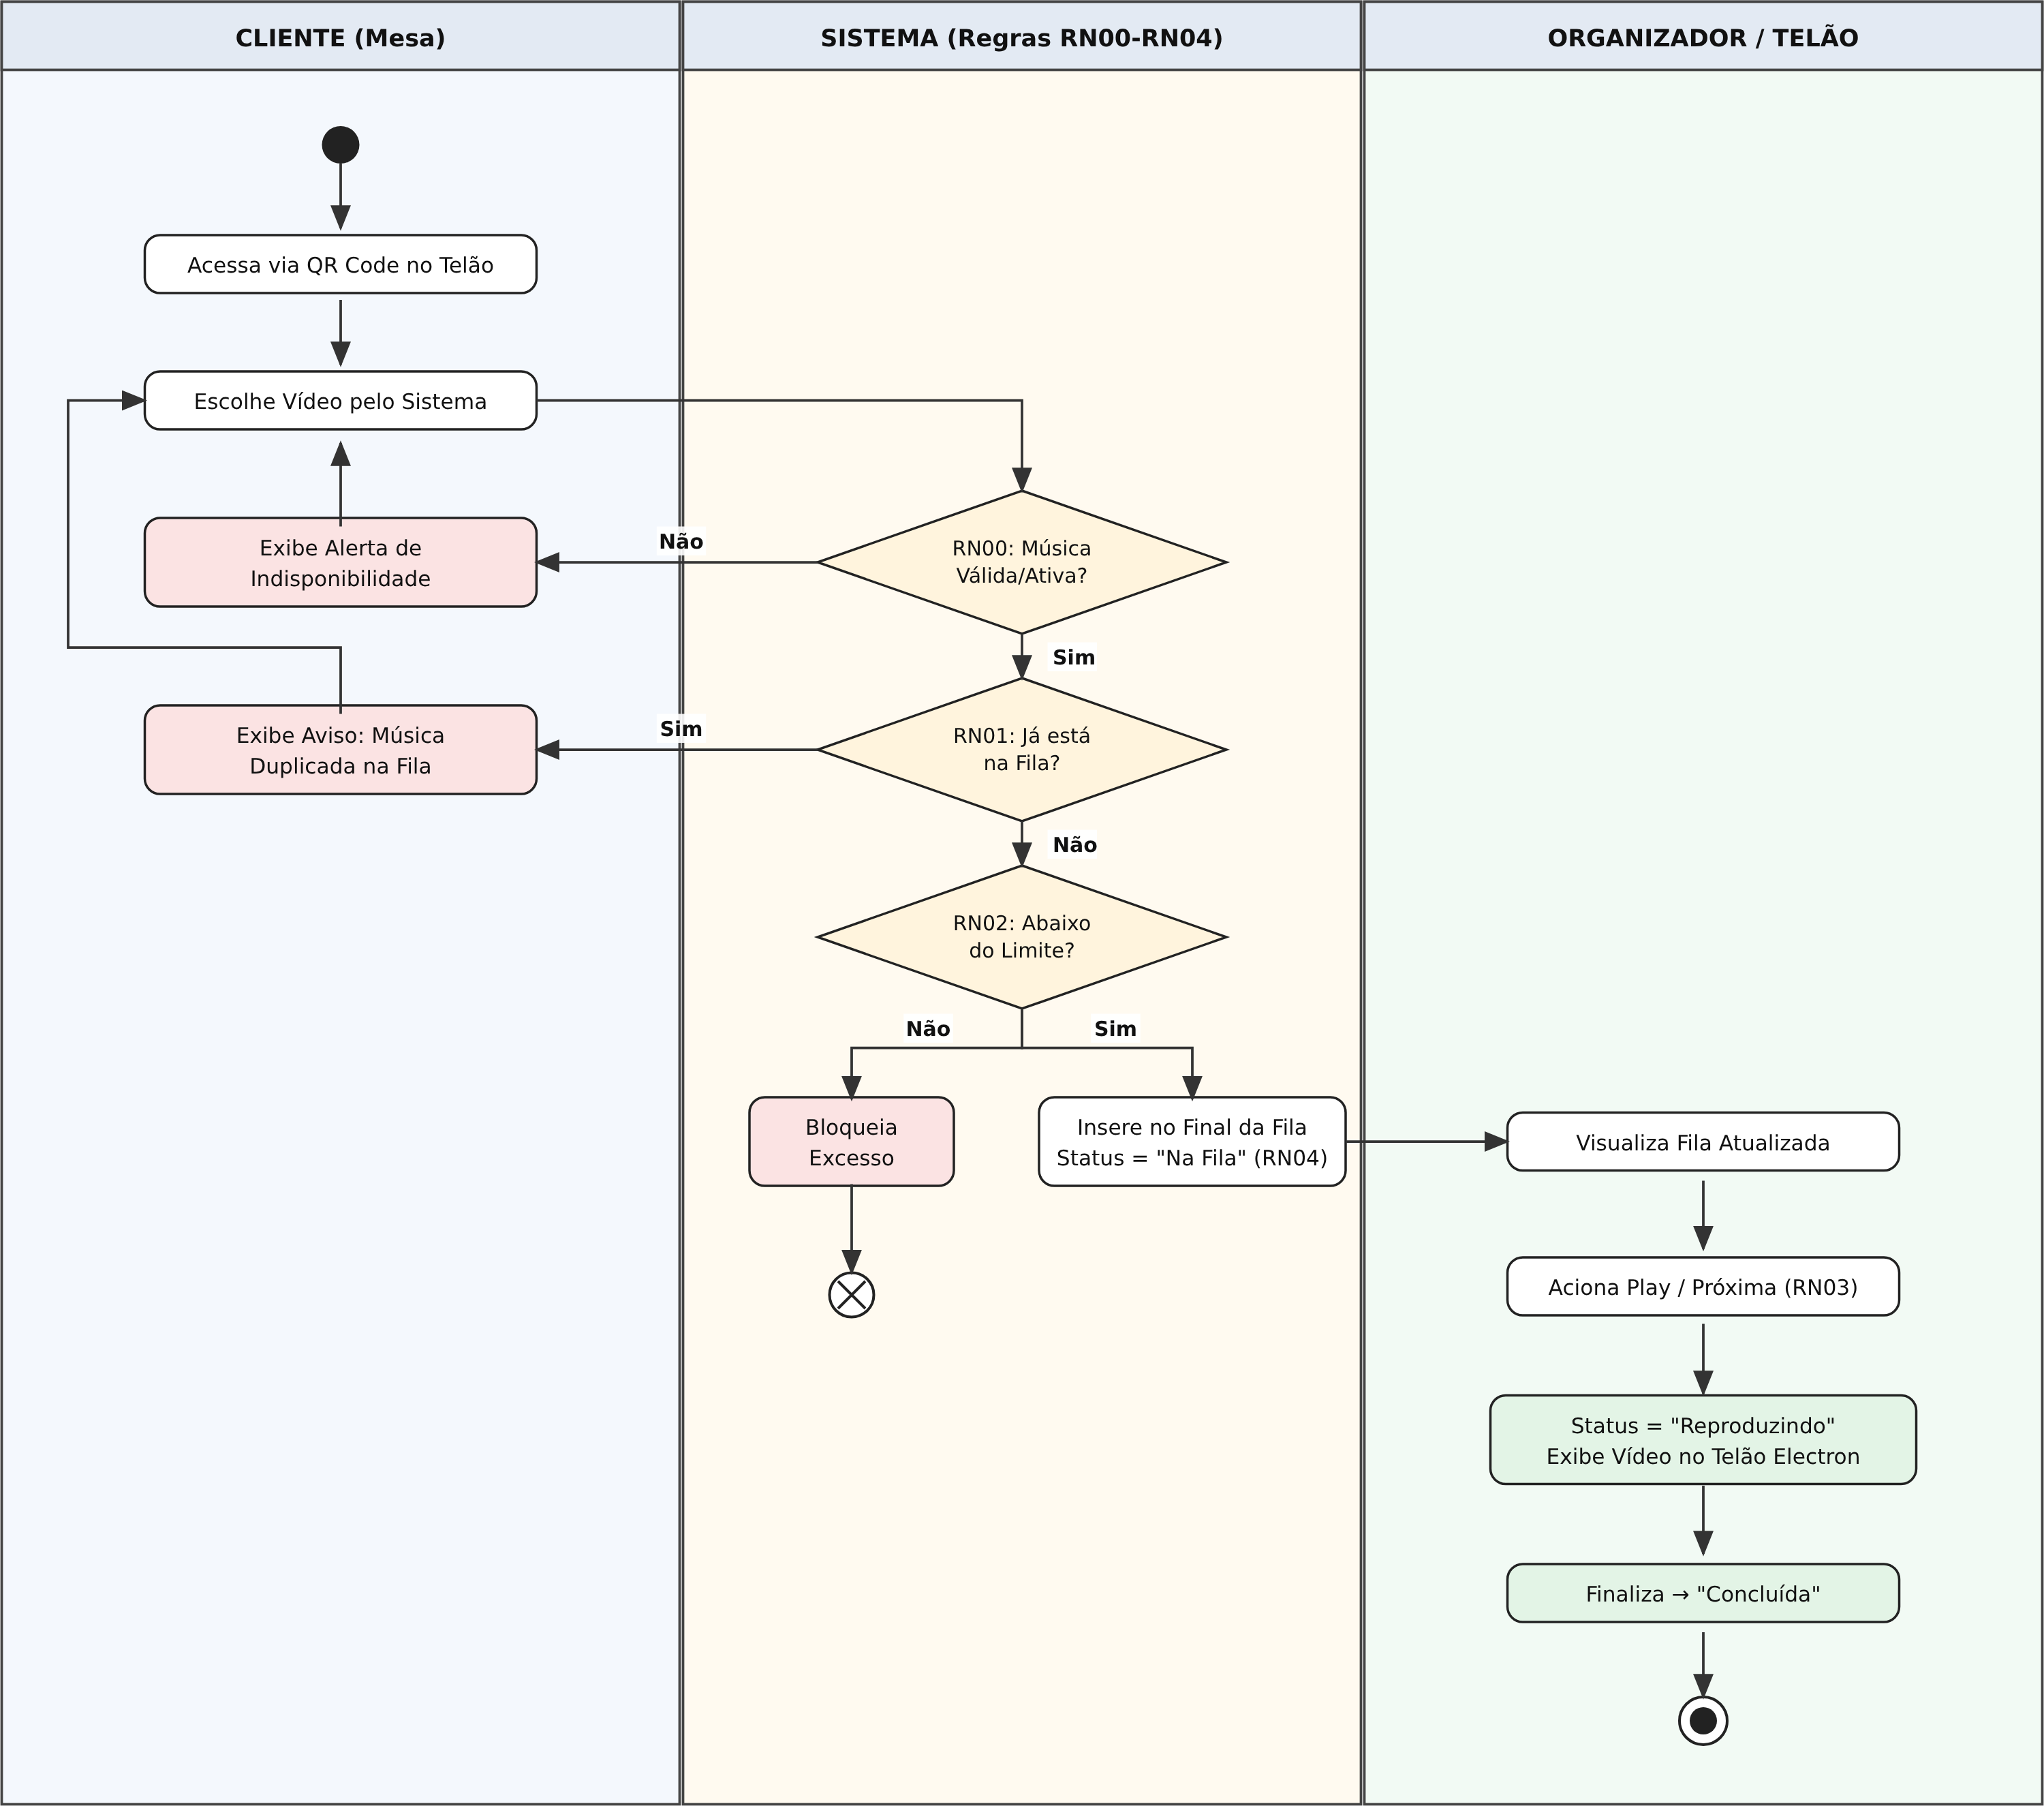
\includegraphics[width=0.95\textwidth,height=0.78\textheight,keepaspectratio]{imagens/diagrama_atividades.png}
\end{center}
\legend{Fonte: Elaborado pelos autores (2026).}
\end{figure}

%% -------------------------------------------------------------------------- %%

% !TEX root = ../documento.tex
%% ========================================================================== %%
%% Capítulo 3 - Análise do Sistema (versão revisada para comparação)         %%
%% ========================================================================== %%

\chapter{Análise do Sistema} \label{cap:analise-revisado}

Este capítulo transforma a compreensão do contexto operacional do Apache Gru Rock Bar e das necessidades identificadas em uma visão estruturada do sistema \textbf{Karaokê Apache}. O objetivo é definir o que o sistema deve fazer, quem interage com ele, quais conceitos compõem seu domínio, quais requisitos devem ser atendidos e quais restrições condicionam seu desenvolvimento e sua operação.

A análise mantém o foco no comportamento esperado do sistema e nas regras do negócio. As decisões relacionadas à arquitetura, às tecnologias, à organização dos componentes e aos detalhes de implementação são apresentadas nos capítulos posteriores.

\section{Visão Geral do Sistema}

O sistema \textbf{Karaokê Apache} foi concebido como uma plataforma distribuída centrada na orquestração da fila de reprodução musical. Sua finalidade é substituir o fluxo manual de pedidos por um processo organizado, no qual o cliente solicita uma música, acompanha a fila e aguarda sua vez, enquanto o organizador administra as apresentações e controla a reprodução da música ativa no telão.

O sistema possui três áreas funcionais principais:

\begin{itemize}
  \item \textbf{Solicitação de músicas:} permite que o cliente se identifique, pesquise uma música disponível e solicite sua inclusão na fila;
  \item \textbf{Administração da fila:} permite que o organizador acompanhe, ordene, inicie, avance ou remova pedidos;
  \item \textbf{Exibição da apresentação:} atualiza instantaneamente o estado da música ativa para que o reprodutor desktop dedicado renderize o vídeo correspondente em tela cheia na TV do bar.
\end{itemize}

O limite do sistema começa no acesso do cliente à interface de solicitação e termina na atualização do estado do pedido e na exibição da música ativa. O sistema não substitui a atuação do organizador, o equipamento de áudio ou a operação artística do evento. Também não é responsável pela produção do conteúdo audiovisual nem pela disponibilidade dos vídeos de terceiros.

\section{Atores Envolvidos}

Foram identificados três atores que interagem diretamente com o sistema ou com seus resultados. Os gestores do estabelecimento são partes interessadas do projeto, mas não constituem um ator operacional separado quando utilizam as mesmas funcionalidades do administrador.

\begin{table}[H]
\IBGEtab{%
  \caption{Atores envolvidos no sistema Karaokê Apache.}%
  \label{tab:atores-revisado}%
}{%
  \footnotesize
  \begin{tabularx}{\textwidth}{p{3.5cm}p{2.8cm}X}
    \toprule
    \textbf{Ator} & \textbf{Tipo} & \textbf{Papel no sistema} \\
    \midrule
    \textbf{Cliente (Cantor)} & Humano, primário & Identifica-se no sistema, pesquisa uma música, solicita sua inclusão na fila e acompanha a posição do pedido e a música em execução. \\
    \addlinespace
    \textbf{Administrador (Organizador)} & Humano, primário & Controla a operação do karaokê, inicia apresentações, avança a fila, remove pedidos e acompanha o estado geral do evento. \\
    \addlinespace
    \textbf{Reprodutor de Telão} & Sistema externo, secundário & Recebe a indicação da música ativa e apresenta o conteúdo audiovisual no telão. \\
    \bottomrule
  \end{tabularx}%
}{%
  \fonte{Elaborado pelos autores (2026).}
}
\end{table}

\section{Casos de Uso}

Os casos de uso descrevem as funcionalidades sob a perspectiva dos atores e representam os comportamentos relevantes para a operação do sistema. O diagrama da Figura \ref{fig:casos_uso-revisado} apresenta a relação entre os atores e os casos de uso principais.

\begin{figure}[H]
  \caption{Diagrama de Casos de Uso UML do sistema Karaokê Apache.}
  \label{fig:casos_uso-revisado}
  \begin{center}
    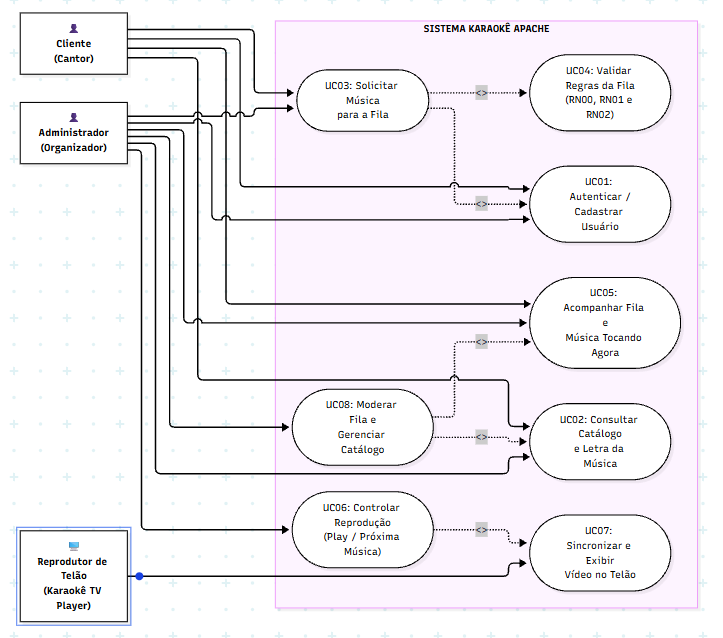
\includegraphics[width=0.92\textwidth]{imagens/DiagramaCasoDeUso.png}
  \end{center}
  \legend{Fonte: Elaborado pelos autores (2026).}
\end{figure}

Os casos de uso foram organizados conforme a necessidade que atendem. O caso de uso UC04 é incluído por UC03, pois suas validações fazem parte da solicitação de uma música. O caso de uso UC07 representa a comunicação do estado da fila com o reprodutor de telão, sem definir a tecnologia utilizada para essa comunicação.

\begin{table}[H]
\IBGEtab{%
  \caption{Visão geral dos casos de uso do sistema Karaokê Apache.}%
  \label{tab:casos_uso-revisado}%
}{%
  \footnotesize
  \begin{tabularx}{\textwidth}{p{1.2cm}p{3.2cm}p{2.5cm}X}
    \toprule
    \textbf{Código} & \textbf{Caso de uso} & \textbf{Atores} & \textbf{Objetivo e fluxo principal} \\
    \midrule
    UC01 & Identificar participante & Cliente, Administrador & O ator informa os dados necessários para acessar as funcionalidades correspondentes ao seu perfil. O sistema valida a identificação e apresenta a área autorizada. \\
    \addlinespace
    UC02 & Pesquisar e escolher música & Cliente, Administrador & O ator informa título ou artista, consulta os resultados disponíveis e seleciona uma música para continuar a solicitação. \\
    \addlinespace
    UC03 & Solicitar música para a fila & Cliente & O cliente confirma a música escolhida. O sistema executa UC04 e, se as regras forem atendidas, registra o pedido no final da fila. \\
    \addlinespace
    UC04 & Validar solicitação de música & Sistema, incluído em UC03 & O sistema verifica a disponibilidade da música, a existência de duplicidade e o limite de pedidos ativos do participante. Em caso de falha, rejeita a solicitação e informa o motivo. \\
    \addlinespace
    UC05 & Acompanhar fila e música atual & Cliente, Administrador & O ator visualiza a música em execução, os próximos pedidos e a posição dos itens na fila. \\
    \addlinespace
    UC06 & Controlar apresentação & Administrador & O organizador inicia um pedido, encerra a apresentação atual ou avança para o próximo item, atualizando o estado da fila. \\
    \addlinespace
    UC07 & Atualizar exibição do telão & Reprodutor de Telão & O sistema informa a música ativa e o reprodutor apresenta o conteúdo correspondente. Quando não há música ativa, o telão exibe o estado de espera. \\
    \addlinespace
    UC08 & Moderar fila & Administrador & O organizador remove um pedido, limpa a fila ao encerrar o evento ou corrige uma situação excepcional conforme as regras do estabelecimento. \\
    \bottomrule
  \end{tabularx}%
}{%
  \fonte{Elaborado pelos autores (2026).}
}
\end{table}

\section{Modelo Conceitual}

O modelo conceitual representa os principais conceitos do domínio e os relacionamentos entre eles, sem definir tecnologias, componentes ou operações de implementação. A Figura \ref{fig:classes_conceitual-revisado} apresenta a representação conceitual do sistema.

\begin{figure}[H]
  \caption{Diagrama de Classes Conceitual UML do sistema Karaokê Apache.}
  \label{fig:classes_conceitual-revisado}
  \begin{center}
    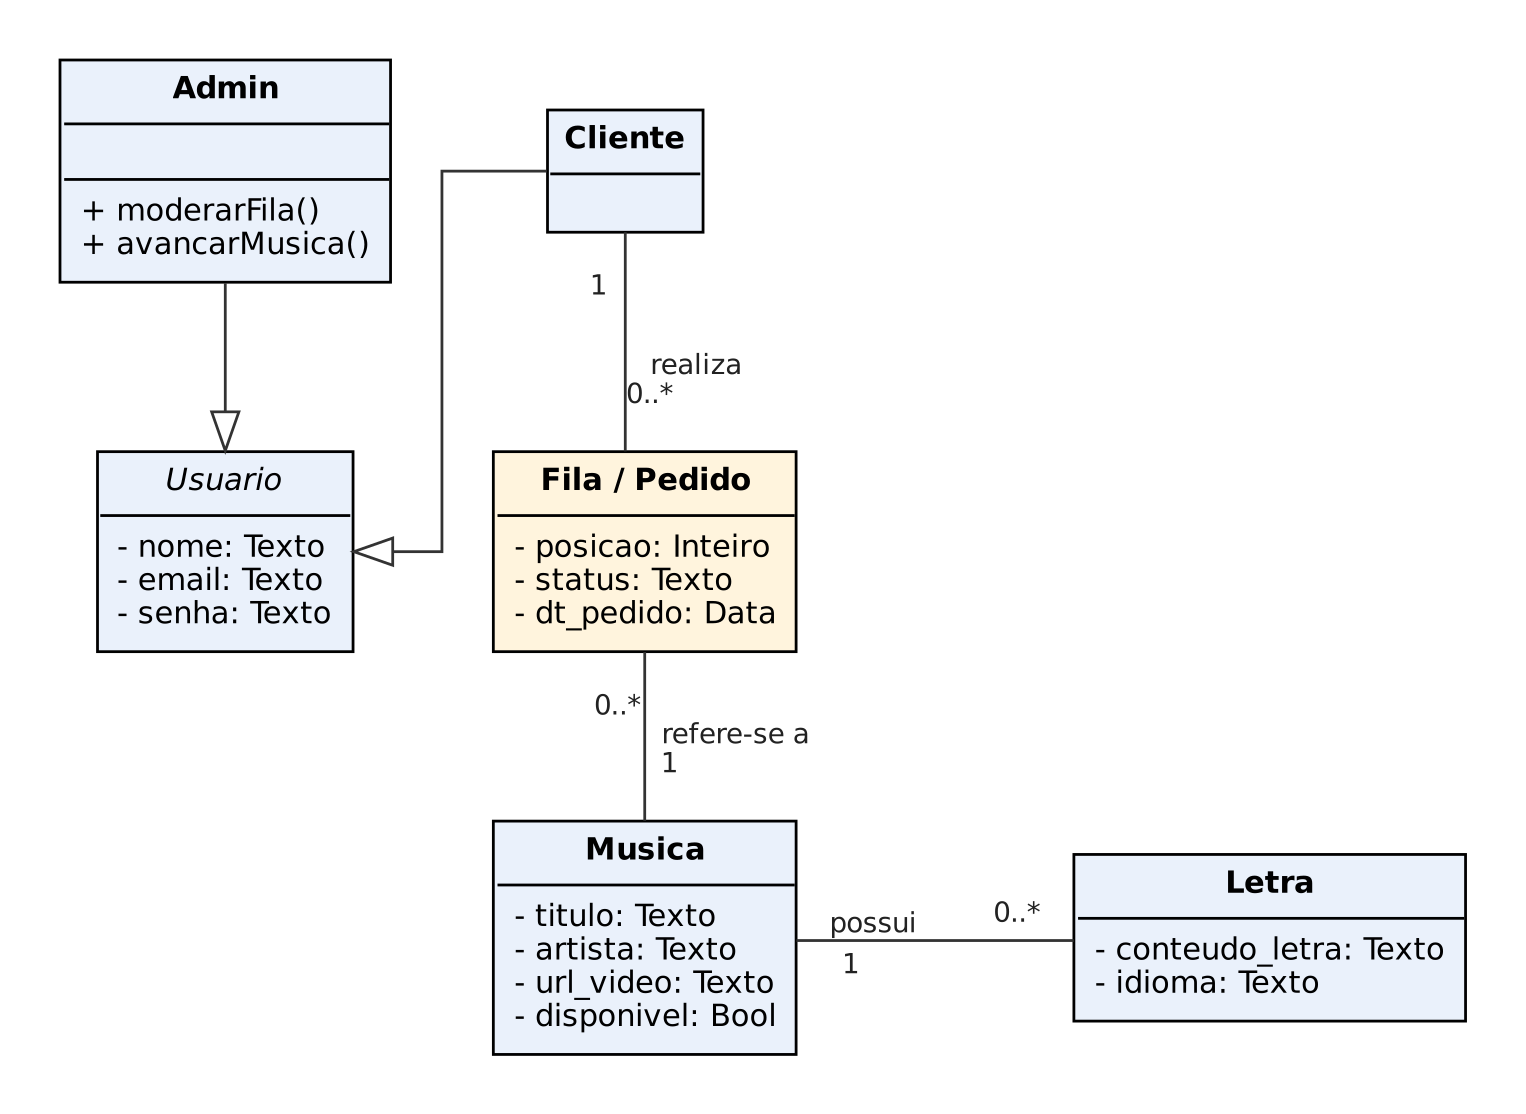
\includegraphics[width=\textwidth,height=0.78\textheight,keepaspectratio]{imagens/diagrama_classes_conceitual.png}
  \end{center}
  \legend{Fonte: Elaborado pelos autores (2026).}
\end{figure}

Os conceitos principais são:

\begin{itemize}
  \item \textbf{Usuário:} representa uma pessoa identificada no sistema. Seus papéis podem ser especializados em \textbf{Cliente} e \textbf{Administrador}, conforme as permissões necessárias para a operação;
  \item \textbf{Cliente:} representa o participante que solicita músicas e acompanha a fila;
  \item \textbf{Administrador:} representa o organizador responsável pelo controle das apresentações;
  \item \textbf{Música:} representa uma opção musical disponível para solicitação, com título, artista e referência ao conteúdo audiovisual;
  \item \textbf{Pedido:} representa a solicitação de uma música feita por um cliente, contendo posição, data da solicitação e estado do atendimento;
  \item \textbf{Letra:} representa o conteúdo textual associado a uma música. No escopo atual, é um conceito previsto para evolução futura e não constitui funcionalidade essencial do MVP.
\end{itemize}

As relações fundamentais do domínio são: um cliente pode realizar vários pedidos; cada pedido é realizado por um único cliente; cada pedido refere-se a uma música; uma música pode ser referenciada por vários pedidos ao longo de diferentes sessões; e cada pedido possui um estado pertencente ao ciclo de atendimento definido pelas regras de negócio.

\section{Requisitos Funcionais}

Os requisitos funcionais especificam os serviços e comportamentos que o sistema deverá oferecer para atender às necessidades N01 a N04 identificadas no contexto do projeto.

\begin{table}[H]
\IBGEtab{%
  \caption{Requisitos funcionais do sistema Karaokê Apache.}%
  \label{tab:requisitos_funcionais-revisado}%
}{%
  \footnotesize
  \begin{tabularx}{\textwidth}{p{1.3cm}p{3.4cm}X p{1.8cm}}
    \toprule
    \textbf{Código} & \textbf{Requisito} & \textbf{Descrição} & \textbf{Prioridade} \\
    \midrule
    RF01 & Identificação de usuário & Permitir que o participante ou organizador se identifique e receba acesso às funcionalidades correspondentes ao seu papel. & Média \\
    \addlinespace
    RF02 & Pesquisa de músicas & Permitir a pesquisa de músicas por título ou artista. & Alta \\
    \addlinespace
    RF03 & Seleção de música & Permitir que o usuário selecione uma música entre os resultados disponíveis. & Alta \\
    \addlinespace
    RF04 & Inclusão de pedido & Permitir que o cliente confirme uma música e inclua o pedido no final da fila. & Alta \\
    \addlinespace
    RF05 & Validação do pedido & Validar disponibilidade, duplicidade e limite de pedidos antes da inclusão na fila. & Alta \\
    \addlinespace
    RF06 & Acompanhamento da fila & Exibir a música ativa, os próximos pedidos e a posição dos itens na fila. & Alta \\
    \addlinespace
    RF07 & Início de apresentação & Permitir que o administrador inicie a apresentação de um pedido selecionado. & Alta \\
    \addlinespace
    RF08 & Avanço da fila & Permitir que o administrador encerre a apresentação atual e avance para o próximo pedido. & Alta \\
    \addlinespace
    RF09 & Moderação de pedidos & Permitir que o administrador remova pedidos individuais ou limpe a fila ao final do evento. & Alta \\
    \addlinespace
    RF10 & Exibição da música ativa & Apresentar no telão a música atualmente em execução e um estado de espera quando não houver apresentação. & Alta \\
    \addlinespace
    RF11 & Atualização do estado do pedido & Registrar as transições entre os estados \textit{Na Fila}, \textit{Reproduzindo}, \textit{Concluído} e \textit{Cancelado}. & Alta \\
    \addlinespace
    RF12 & Feedback das operações & Informar o resultado das ações realizadas, incluindo confirmações, falhas de validação e indisponibilidade de conexão. & Alta \\
    \bottomrule
  \end{tabularx}%
}{%
  \fonte{Elaborado pelos autores (2026).}
}
\end{table}

\subsection{Critérios de aceitação dos requisitos centrais}

Os requisitos centrais devem ser verificáveis por meio de cenários de uso. A Tabela \ref{tab:criterios_aceitacao-revisado} apresenta critérios de aceitação iniciais para o MVP.

\begin{table}[H]
\IBGEtab{%
  \caption{Critérios de aceitação dos requisitos centrais.}%
  \label{tab:criterios_aceitacao-revisado}%
}{%
  \footnotesize
  \begin{tabularx}{\textwidth}{p{1.5cm}X}
    \toprule
    \textbf{Req.} & \textbf{Critério de aceitação} \\
    \midrule
    RF04/RF05 & Dado que a música esteja disponível e não esteja duplicada, ao confirmar a solicitação o sistema deverá criar um pedido na última posição da fila. \\
    \addlinespace
    RF05 & Dado que a música já esteja na fila ou em reprodução, ao tentar solicitá-la novamente o sistema deverá rejeitar o pedido e informar o motivo. \\
    \addlinespace
    RF06 & Dado que existam pedidos ativos, ao acessar a fila o usuário deverá visualizar a música atual e a ordem dos próximos pedidos. \\
    \addlinespace
    RF07/RF08 & Dado que o administrador inicie ou avance uma apresentação, o estado do pedido deverá ser atualizado e o próximo item deverá assumir a condição correspondente. \\
    \addlinespace
    RF10 & Dado que exista uma música ativa, o reprodutor deverá apresentar o conteúdo correspondente no telão; sem música ativa, deverá apresentar o estado de espera. \\
    \addlinespace
    RF12 & Dado que uma operação seja rejeitada ou concluída, o sistema deverá apresentar uma mensagem que permita ao usuário compreender o resultado. \\
    \bottomrule
  \end{tabularx}%
}{%
  \fonte{Elaborado pelos autores (2026).}
}
\end{table}

\section{Requisitos Não Funcionais}

Os requisitos não funcionais definem características de qualidade e condições de operação que complementam os requisitos funcionais. Eles devem ser validados posteriormente por testes, inspeções ou análise da documentação técnica.

\begin{table}[H]
\IBGEtab{%
  \caption{Requisitos não funcionais do sistema Karaokê Apache.}%
  \label{tab:requisitos_nao_funcionais-revisado}%
}{%
  \footnotesize
  \begin{tabularx}{\textwidth}{p{1.4cm}p{2.6cm}p{3.4cm}X}
    \toprule
    \textbf{Código} & \textbf{Categoria} & \textbf{Requisito} & \textbf{Critério esperado} \\
    \midrule
    RNF01 & Usabilidade & Acesso simples em dispositivos móveis & O cliente deverá conseguir acessar a solicitação sem instalar um aplicativo adicional e concluir o fluxo com poucas etapas. \\
    \addlinespace
    RNF02 & Usabilidade & Legibilidade em ambiente noturno & As informações essenciais deverão apresentar contraste e tamanho adequados para o uso em um bar com pouca iluminação. \\
    \addlinespace
    RNF03 & Desempenho & Atualização da fila & Uma alteração de estado deverá ser refletida nos participantes e no telão em tempo compatível com a operação do evento, com meta de até dois segundos na rede local. \\
    \addlinespace
    RNF04 & Compatibilidade & Acesso por navegadores comuns & A interface do cliente deverá funcionar nas versões atuais dos principais navegadores para dispositivos móveis. \\
    \addlinespace
    RNF05 & Segurança & Controle de acesso & Apenas o administrador poderá executar ações de controle da fila e da apresentação. \\
    \addlinespace
    RNF06 & Segurança e privacidade & Proteção dos dados pessoais & A coleta deverá limitar-se aos dados necessários para identificar o participante e operar a fila. \\
    \addlinespace
    RNF07 & Confiabilidade & Consistência dos estados & O sistema não deverá permitir transições incompatíveis ou perda da ordem dos pedidos durante uma operação normal. \\
    \addlinespace
    RNF08 & Manutenibilidade & Separação de responsabilidades & A solução deverá manter separadas as responsabilidades de identificação, pedidos, fila, reprodução e administração. \\
    \bottomrule
  \end{tabularx}%
}{%
  \fonte{Elaborado pelos autores (2026).}
}
\end{table}

\section{Restrições do Sistema}

O desenvolvimento e a operação do sistema estão sujeitos às seguintes restrições:

\begin{itemize}
  \item \textbf{Dependência de conectividade:} os participantes e o equipamento de exibição dependem de conexão adequada durante o evento para consultar a fila, atualizar estados e acessar o conteúdo audiovisual;
  \item \textbf{Disponibilidade de conteúdo de terceiros:} determinados conteúdos podem não permitir reprodução no ambiente utilizado, o que pode impedir ou interromper a apresentação de uma música;
  \item \textbf{Infraestrutura existente:} a solução deve operar com os equipamentos disponíveis no estabelecimento, incluindo dispositivos móveis dos clientes, computador de controle, telão e sistema de som;
  \item \textbf{Restrição orçamentária:} o projeto deve evitar custos de licenciamento incompatíveis com a realidade do estabelecimento parceiro;
  \item \textbf{Proteção de dados pessoais:} a coleta, o armazenamento e o uso de dados dos participantes devem observar os princípios da Lei Geral de Proteção de Dados Pessoais (LGPD), especialmente necessidade, finalidade e transparência \cite{brasil2018lgpd};
  \item \textbf{Regras operacionais do evento:} a ordem dos pedidos, o limite de solicitações por participante e as ações de moderação devem respeitar as políticas definidas pelo organizador karaokê.
\end{itemize}

\subsection{Rastreabilidade entre necessidades, regras e requisitos}

A Tabela \ref{tab:rastreabilidade-revisado} relaciona as necessidades identificadas no contexto às regras de negócio, aos casos de uso e aos requisitos funcionais correspondentes.

\begin{table}[H]
\IBGEtab{%
  \caption{Matriz de rastreabilidade da análise do sistema.}%
  \label{tab:rastreabilidade-revisado}%
}{%
  \footnotesize
  \begin{tabularx}{\textwidth}{p{1.2cm}p{3.0cm}p{2.0cm}p{2.0cm}X}
    \toprule
    \textbf{Nec.} & \textbf{Necessidade} & \textbf{Regras} & \textbf{Casos de uso} & \textbf{Requisitos funcionais} \\
    \midrule
    N01 & Escolha de música pelo próprio sistema & RN00 & UC01, UC02, UC03, UC04 & RF01 a RF05 \\
    \addlinespace
    N02 & Transparência da fila & RN04 & UC05, UC07 & RF06, RF10, RF11, RF12 \\
    \addlinespace
    N03 & Prevenção de repetições e rotatividade & RN01, RN02 & UC03, UC04, UC06, UC08 & RF04, RF05, RF07 a RF09, RF11 \\
    \addlinespace
    N04 & Automação da reprodução no telão & RN03, RN04 & UC06, UC07, UC08 & RF07 a RF12 \\
    \bottomrule
  \end{tabularx}%
}{%
  \fonte{Elaborado pelos autores (2026).}
}
\end{table}

%% -------------------------------------------------------------------------- %%

\chapter{Projeto do Sistema} \label{cap:projeto}

Este capítulo estabelece a especificação técnica da solução \textbf{Karaokê Apache}, transformando o modelo conceitual e os requisitos da análise em uma definição detalhada da arquitetura distribuída, dos componentes de software, do modelo lógico e físico de dados, do projeto das interfaces de usuário, das interações dinâmicas, das tecnologias adotadas e dos mecanismos de segurança.

\section{Arquitetura do Sistema}

A arquitetura do sistema \textbf{Karaokê Apache} foi elaborada a partir dos artefatos de engenharia \texttt{ideia.png} e \texttt{Desenho da Aplicação}, estruturando a solução em quatro subsistemas integrados: \textbf{Cliente Web}, \textbf{Admin Web}, \textbf{API Orquestradora} (conectada ao \textbf{Banco de Dados Relacional}) e o reprodutor desktop \textbf{Electron (Karaokê TV Player)}.

Seguindo os princípios de desacoplamento arquitetural descritos por Sommerville \cite{sommerville2019}, Fowler \cite{fowler2006} e Pressman e Maxim \cite{pressman2016}, a camada de apresentação web e o reprodutor de telão permanecem separados da lógica de persistência, comunicando-se por meio de contratos bem definidos. Na modelagem formal realizada pela equipe na ferramenta UMLet (arquivos \texttt{diagrama\_de\_componentes.uxf} e \texttt{diagrama\_de\_componentes.png}), a arquitetura lógica é organizada em quatro componentes principais (\textbf{Usuários}, \textbf{Fila}, \textbf{Pedido de Música} e \textbf{Reprodutor}), representados no \textbf{Diagrama de Componentes UML} da Figura \ref{fig:uml_componentes}.

\begin{figure}[H]
  \caption{Diagrama de Componentes UML (\texttt{diagrama\_de\_componentes.png}).}
  \label{fig:uml_componentes}
  \begin{center}
    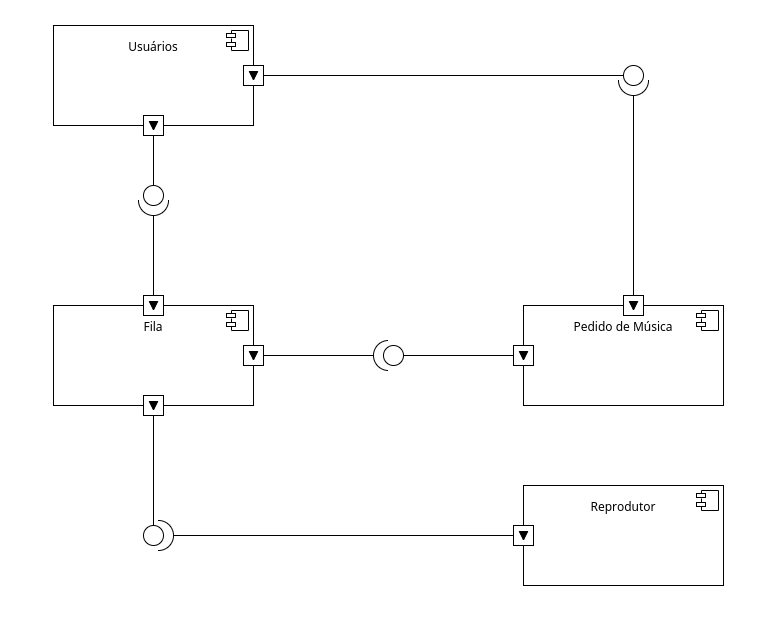
\includegraphics[width=0.88\textwidth]{imagens/diagrama_de_componentes.png}
  \end{center}
  \legend{Fonte: Elaborado pelos autores no software UMLet (2026).}
\end{figure}

\section{Projeto dos Componentes}

Cada componente definido na arquitetura possui responsabilidades coesas e interfaces explícitas de comunicação, detalhadas na Tabela \ref{tab:componentes_uml}:

\begin{table}[H]
\IBGEtab{%
  \caption{Detalhamento técnico dos componentes arquiteturais e suas interfaces.}%
  \label{tab:componentes_uml}%
}{%
  \footnotesize
  \begin{tabularx}{\textwidth}{p{3.0cm}p{4.2cm}X}
    \toprule
    \textbf{Componente} & \textbf{Interfaces (Fornecidas / Requeridas)} & \textbf{Estrutura Interna e Responsabilidades} \\
    \midrule
    \texttt{Usuários} & Fornece: \texttt{IAutenticacao}, \texttt{IPerfilUsuario} & Responsável pelo cadastro, autenticação e diferenciação de permissões entre os papéis \texttt{cliente} (frequentador da mesa) e \texttt{admin} (organizador do palco). \\
    \addlinespace
    \texttt{Pedido de Música} & Requer: \texttt{IAutenticacao}; Fornece: \texttt{IPedidoMusica} & Responsável pela pesquisa e escolha de vídeos musicais diretamente pelo sistema, identificação do vídeo selecionado e validação de disponibilidade (RN00). \\
    \addlinespace
    \texttt{Fila} & Requer: \texttt{IAutenticacao}, \texttt{IPedidoMusica}; Fornece: \texttt{IControleFila} & Núcleo orquestrador do sistema: gerencia a lista ordenada de pedidos (\texttt{queue}), o item em execução (\texttt{currentSong}), aplica o bloqueio de duplicidade (RN01) e processa os comandos \textit{Play}, \textit{Próxima}, \textit{Remover} e \textit{Limpar}. \\
    \addlinespace
    \texttt{Reprodutor} & Requer: \texttt{IControleFila} & Materializado pelo aplicativo desktop \textit{Karaokê TV Player} em Electron: escuta continuamente o estado de \texttt{currentSong} e atualiza o player embarcado em tela cheia na TV do bar. \\
    \bottomrule
  \end{tabularx}%
}{%
  \fonte{Elaborado pelos autores a partir de \texttt{diagrama\_de\_componentes.uxf} (2026).}%
}
\end{table}

Para o cálculo de estimativa de espera $W_k$ exibido na fila para o $k$-ésimo pedido ($k \in \{1, 2, \dots, N\}$), o componente \textbf{Fila} considera a duração média por música ($T_{\text{médio}} \approx 4\text{ min}$) e o tempo médio de troca de cantor no palco ($T_{\text{palco}} \approx 0,5\text{ min}$):

\begin{equation}
  W_k = (k - 1) \cdot \left( T_{\text{médio}} + T_{\text{palco}} \right) + T_{\text{restante\_atual}}
  \label{eq:tempo_espera}
\end{equation}

\section{Modelo de Dados}

O projeto de dados converte o modelo conceitual em uma estrutura relacional normalizada, acrescentando chaves primárias artificiais (\texttt{PK}), chaves estrangeiras (\texttt{FK}), tipos físicos de dados e métodos de negócio das classes de domínio (mantendo a estrutura da tabela \texttt{letra} já preparada no banco de dados para a próxima etapa do projeto). O Quadro \ref{quad:classes_projeto} apresenta o \textbf{Diagrama de Classes de Projeto UML}, enquanto a Tabela \ref{tab:dicionario_dados} documenta o Dicionário de Dados relacional.

\Needspace{10.5cm}
\begin{caixa}{Diagrama de Classes de Projeto UML}{quad:classes_projeto}
\begin{center}
  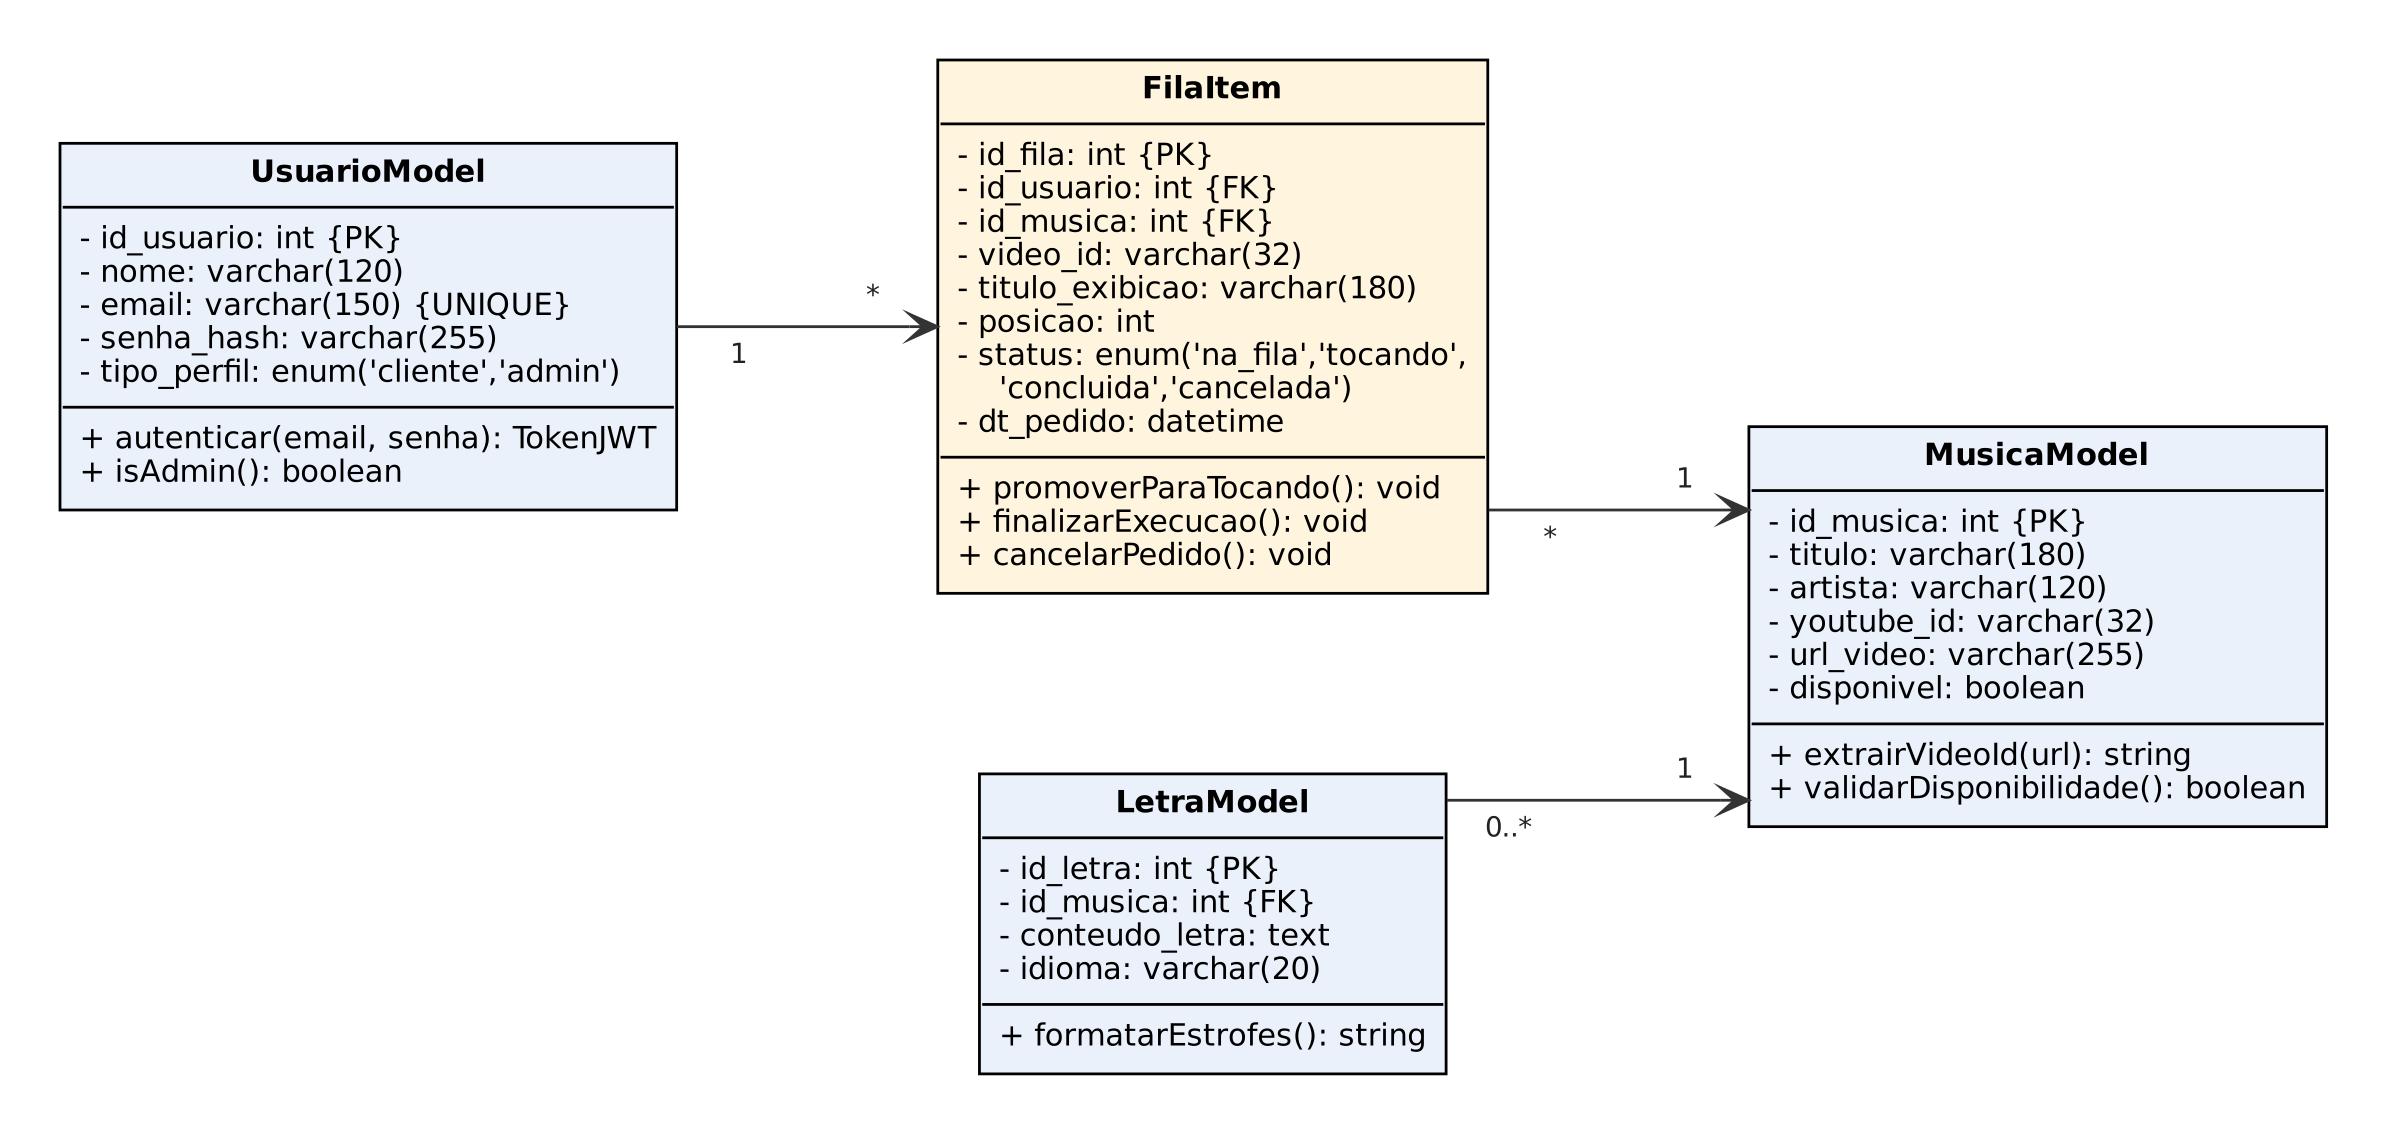
\includegraphics[width=\textwidth,height=0.78\textheight,keepaspectratio]{imagens/diagrama_classes_projeto.png}
\end{center}
\legend{Fonte: Elaborado pelos autores (2026).}
\end{caixa}

\begin{table}[H]
\IBGEtab{%
  \caption{Dicionário de dados do modelo relacional do sistema Karaokê Apache.}%
  \label{tab:dicionario_dados}%
}{%
  \footnotesize
  \begin{tabularx}{\textwidth}{p{2.0cm}p{2.9cm}p{2.7cm}p{2.0cm}X}
    \toprule
    \textbf{Tabela} & \textbf{Atributo} & \textbf{Tipo Físico} & \textbf{Restrições} & \textbf{Descrição no Projeto} \\
    \midrule
    \texttt{usuario} & \texttt{id\_usuario} & \texttt{INT} & \texttt{PK, AI} & Chave primária do usuário. \\
    \texttt{usuario} & \texttt{nome} & \texttt{VARCHAR(120)} & \texttt{NOT NULL} & Nome do participante ou operador. \\
    \texttt{usuario} & \texttt{email} & \texttt{VARCHAR(150)} & \texttt{UNIQUE} & E-mail de login do usuário. \\
    \texttt{usuario} & \texttt{senha\_hash} & \texttt{VARCHAR(255)} & \texttt{NOT NULL} & Senha criptografada (Bcrypt). \\
    \texttt{usuario} & \texttt{tipo\_perfil} & \texttt{ENUM('cliente','admin')} & \texttt{NOT NULL} & Perfil de permissão no sistema. \\
    \midrule
    \texttt{musica} & \texttt{id\_musica} & \texttt{INT} & \texttt{PK, AI} & Identificador único da música. \\
    \texttt{musica} & \texttt{titulo} & \texttt{VARCHAR(180)} & \texttt{NOT NULL} & Nome da música no catálogo. \\
    \texttt{musica} & \texttt{artista} & \texttt{VARCHAR(120)} & \texttt{NOT NULL} & Banda ou intérprete original. \\
    \texttt{musica} & \texttt{youtube\_id} & \texttt{VARCHAR(32)} & \texttt{NOT NULL} & Código de 11 caracteres do YouTube. \\
    \texttt{musica} & \texttt{url\_video} & \texttt{VARCHAR(255)} & \texttt{NOT NULL} & URL completa do vídeo de karaokê. \\
    \texttt{musica} & \texttt{disponivel} & \texttt{BOOLEAN} & \texttt{DEFAULT 1} & Indica se a música está ativa (RN00). \\
    \midrule
    \texttt{letra} & \texttt{id\_letra} & \texttt{INT} & \texttt{PK, AI} & Identificador único da letra. \\
    \texttt{letra} & \texttt{id\_musica} & \texttt{INT} & \texttt{FK, NOT NULL} & Referência à tabela \texttt{musica}. \\
    \texttt{letra} & \texttt{conteudo\_letra} & \texttt{TEXT} & \texttt{NOT NULL} & Letra completa da canção. \\
    \texttt{letra} & \texttt{idioma} & \texttt{VARCHAR(20)} & \texttt{DEFAULT 'pt-BR'} & Idioma da letra cadastrada. \\
    \midrule
    \texttt{fila} & \texttt{id\_fila} & \texttt{INT} & \texttt{PK, AI} & Identificador único do item na fila. \\
    \texttt{fila} & \texttt{id\_usuario} & \texttt{INT} & \texttt{FK, NULL} & Referência ao cliente solicitante. \\
    \texttt{fila} & \texttt{id\_musica} & \texttt{INT} & \texttt{FK, NULL} & Referência à música solicitada. \\
    \texttt{fila} & \texttt{posicao} & \texttt{INT} & \texttt{NOT NULL} & Ordem de chamada na fila ativa. \\
    \texttt{fila} & \texttt{status} & \texttt{ENUM('na\_fila', 'tocando', 'concluida', 'cancelada')} & \texttt{DEFAULT 'na\_fila'} & Estado atual do pedido (RN04). \\
    \texttt{fila} & \texttt{dt\_pedido} & \texttt{DATETIME} & \texttt{DEFAULT NOW()} & Data e hora do registro na fila. \\
    \bottomrule
  \end{tabularx}%
}{%
  \fonte{Elaborado pelos autores a partir de \texttt{Conceitual.brM3} (2026).}%
}
\end{table}

\section{Projeto da Interface do Usuário}

O projeto visual das interfaces do sistema priorizou simplicidade operacional, alto contraste em tema escuro (\textit{Dark Mode}) para uso confortável no ambiente noturno do Apache Gru Rock Bar e separação rigorosa entre a tela de controle e a tela pública do telão:

\begin{enumerate}
  \item \textbf{Interface Web de Controle e Fila (\texttt{Karaokê -- Controle e Fila}):} projetada para execução em navegador web (móvel e desktop), apresenta três blocos visuais empilhados:
    \begin{itemize}
      \item \textit{Bloco de Busca e Escolha de Vídeo:} permite ao usuário pesquisar e escolher o vídeo musical diretamente pelo próprio sistema, acionando o botão \textbf{Adicionar à fila};
      \item \textit{Card ``Tocando Agora'':} painel destacado com indicador luminoso verde em tempo real, exibindo o título e o código da música em execução no palco, acompanhado do botão \textbf{Próxima música};
      \item \textit{Lista ``Fila de Músicas (N)'':} listagem numerada sequencialmente ($1, 2, \dots, N$) com botões de ação rápida para iniciar a faixa (\textbf{Play}), remover um item individual (\textbf{X}) ou acionar \textbf{Limpar fila}.
    \end{itemize}
  \item \textbf{Interface Desktop Nativa (\texttt{Karaokê TV Player} em Electron):} projetada para exibição no telão/projetor do bar (junto ao QR Code de acesso rápido), contém uma barra de status superior minimalista (\textit{``Conectado -- Tocando: [ID\_DO\_VIDEO]''}) e dedica a área principal ao reprodutor de vídeo em tela cheia.
\end{enumerate}

O Quadro \ref{quad:interfaces_mvp} representa a disposição visual (\textit{wireframe} de projeto) das duas interfaces integradas.

\Needspace{11.7cm}
\begin{caixa}{Representação das Interfaces de Usuário (Web Controle/Fila e Electron TV Player)}{quad:interfaces_mvp}
\begin{center}
  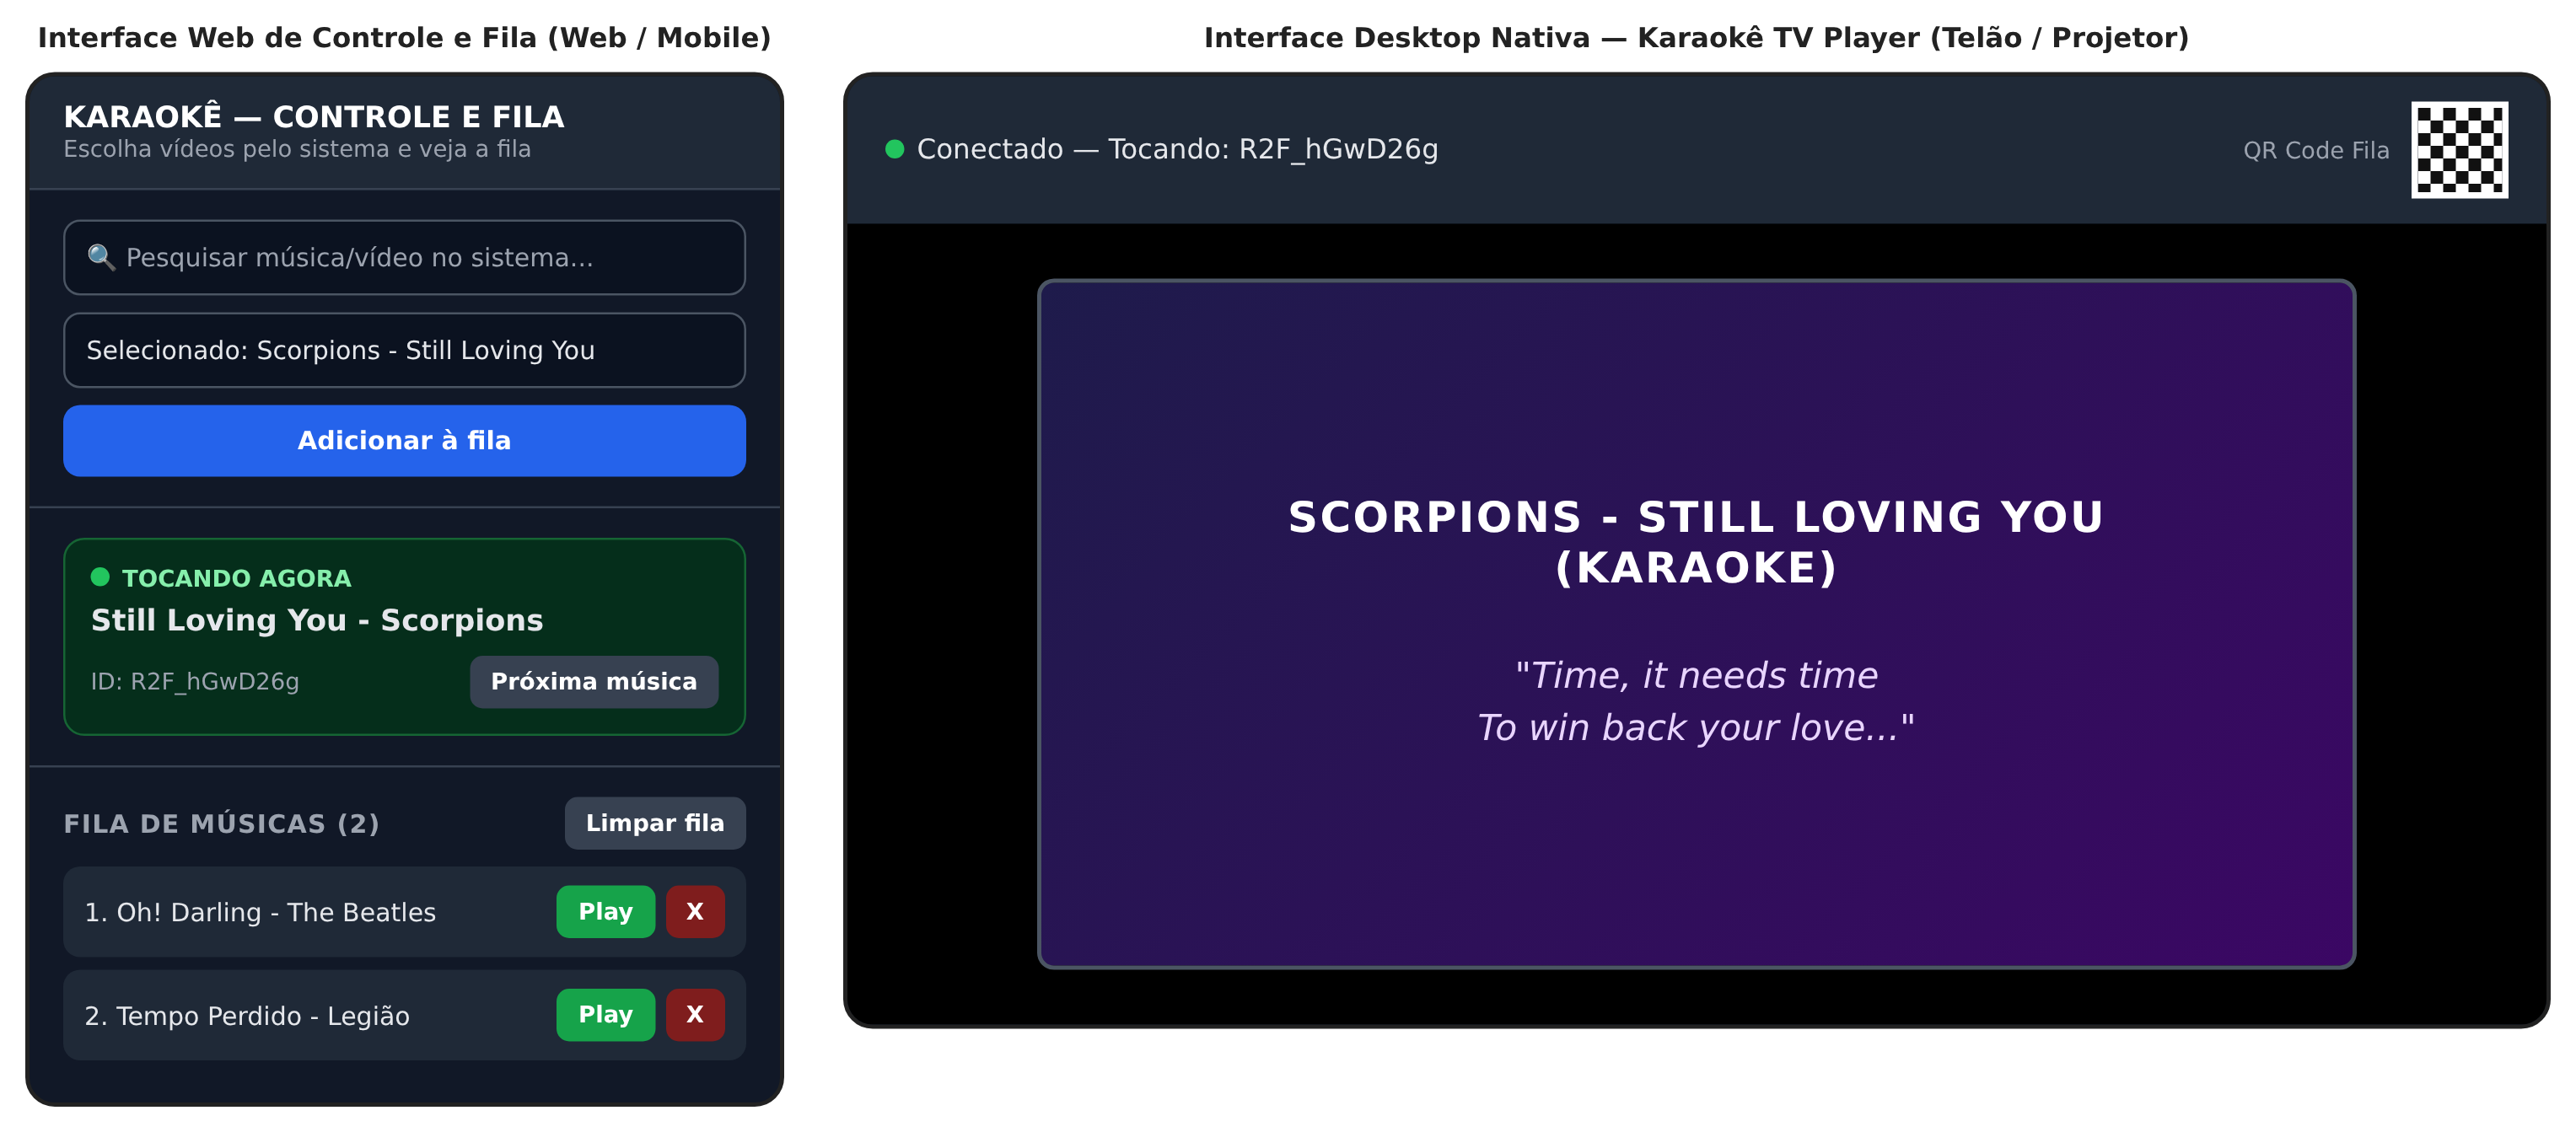
\includegraphics[width=\textwidth,height=0.78\textheight,keepaspectratio]{imagens/wireframe_interfaces.png}
\end{center}
\legend{Fonte: Elaborado pelos autores com base nas telas do projeto e \texttt{Poc.mp4} (2026).}
\end{caixa}

\section{Diagramas de Interação}

Para demonstrar como os objetos e subsistemas colaboram dinamicamente ao longo do tempo para cumprir os requisitos do sistema, o Quadro \ref{quad:sequencia} apresenta o \textbf{Diagrama de Sequência UML} correspondente ao cenário principal de submissão de um pedido musical e seu posterior acionamento para reprodução no telão em Electron.

\Needspace{15.5cm}
\begin{caixa}{Diagrama de Sequência UML -- Submissão de Música e Sincronização com o Telão}{quad:sequencia}
\begin{center}
  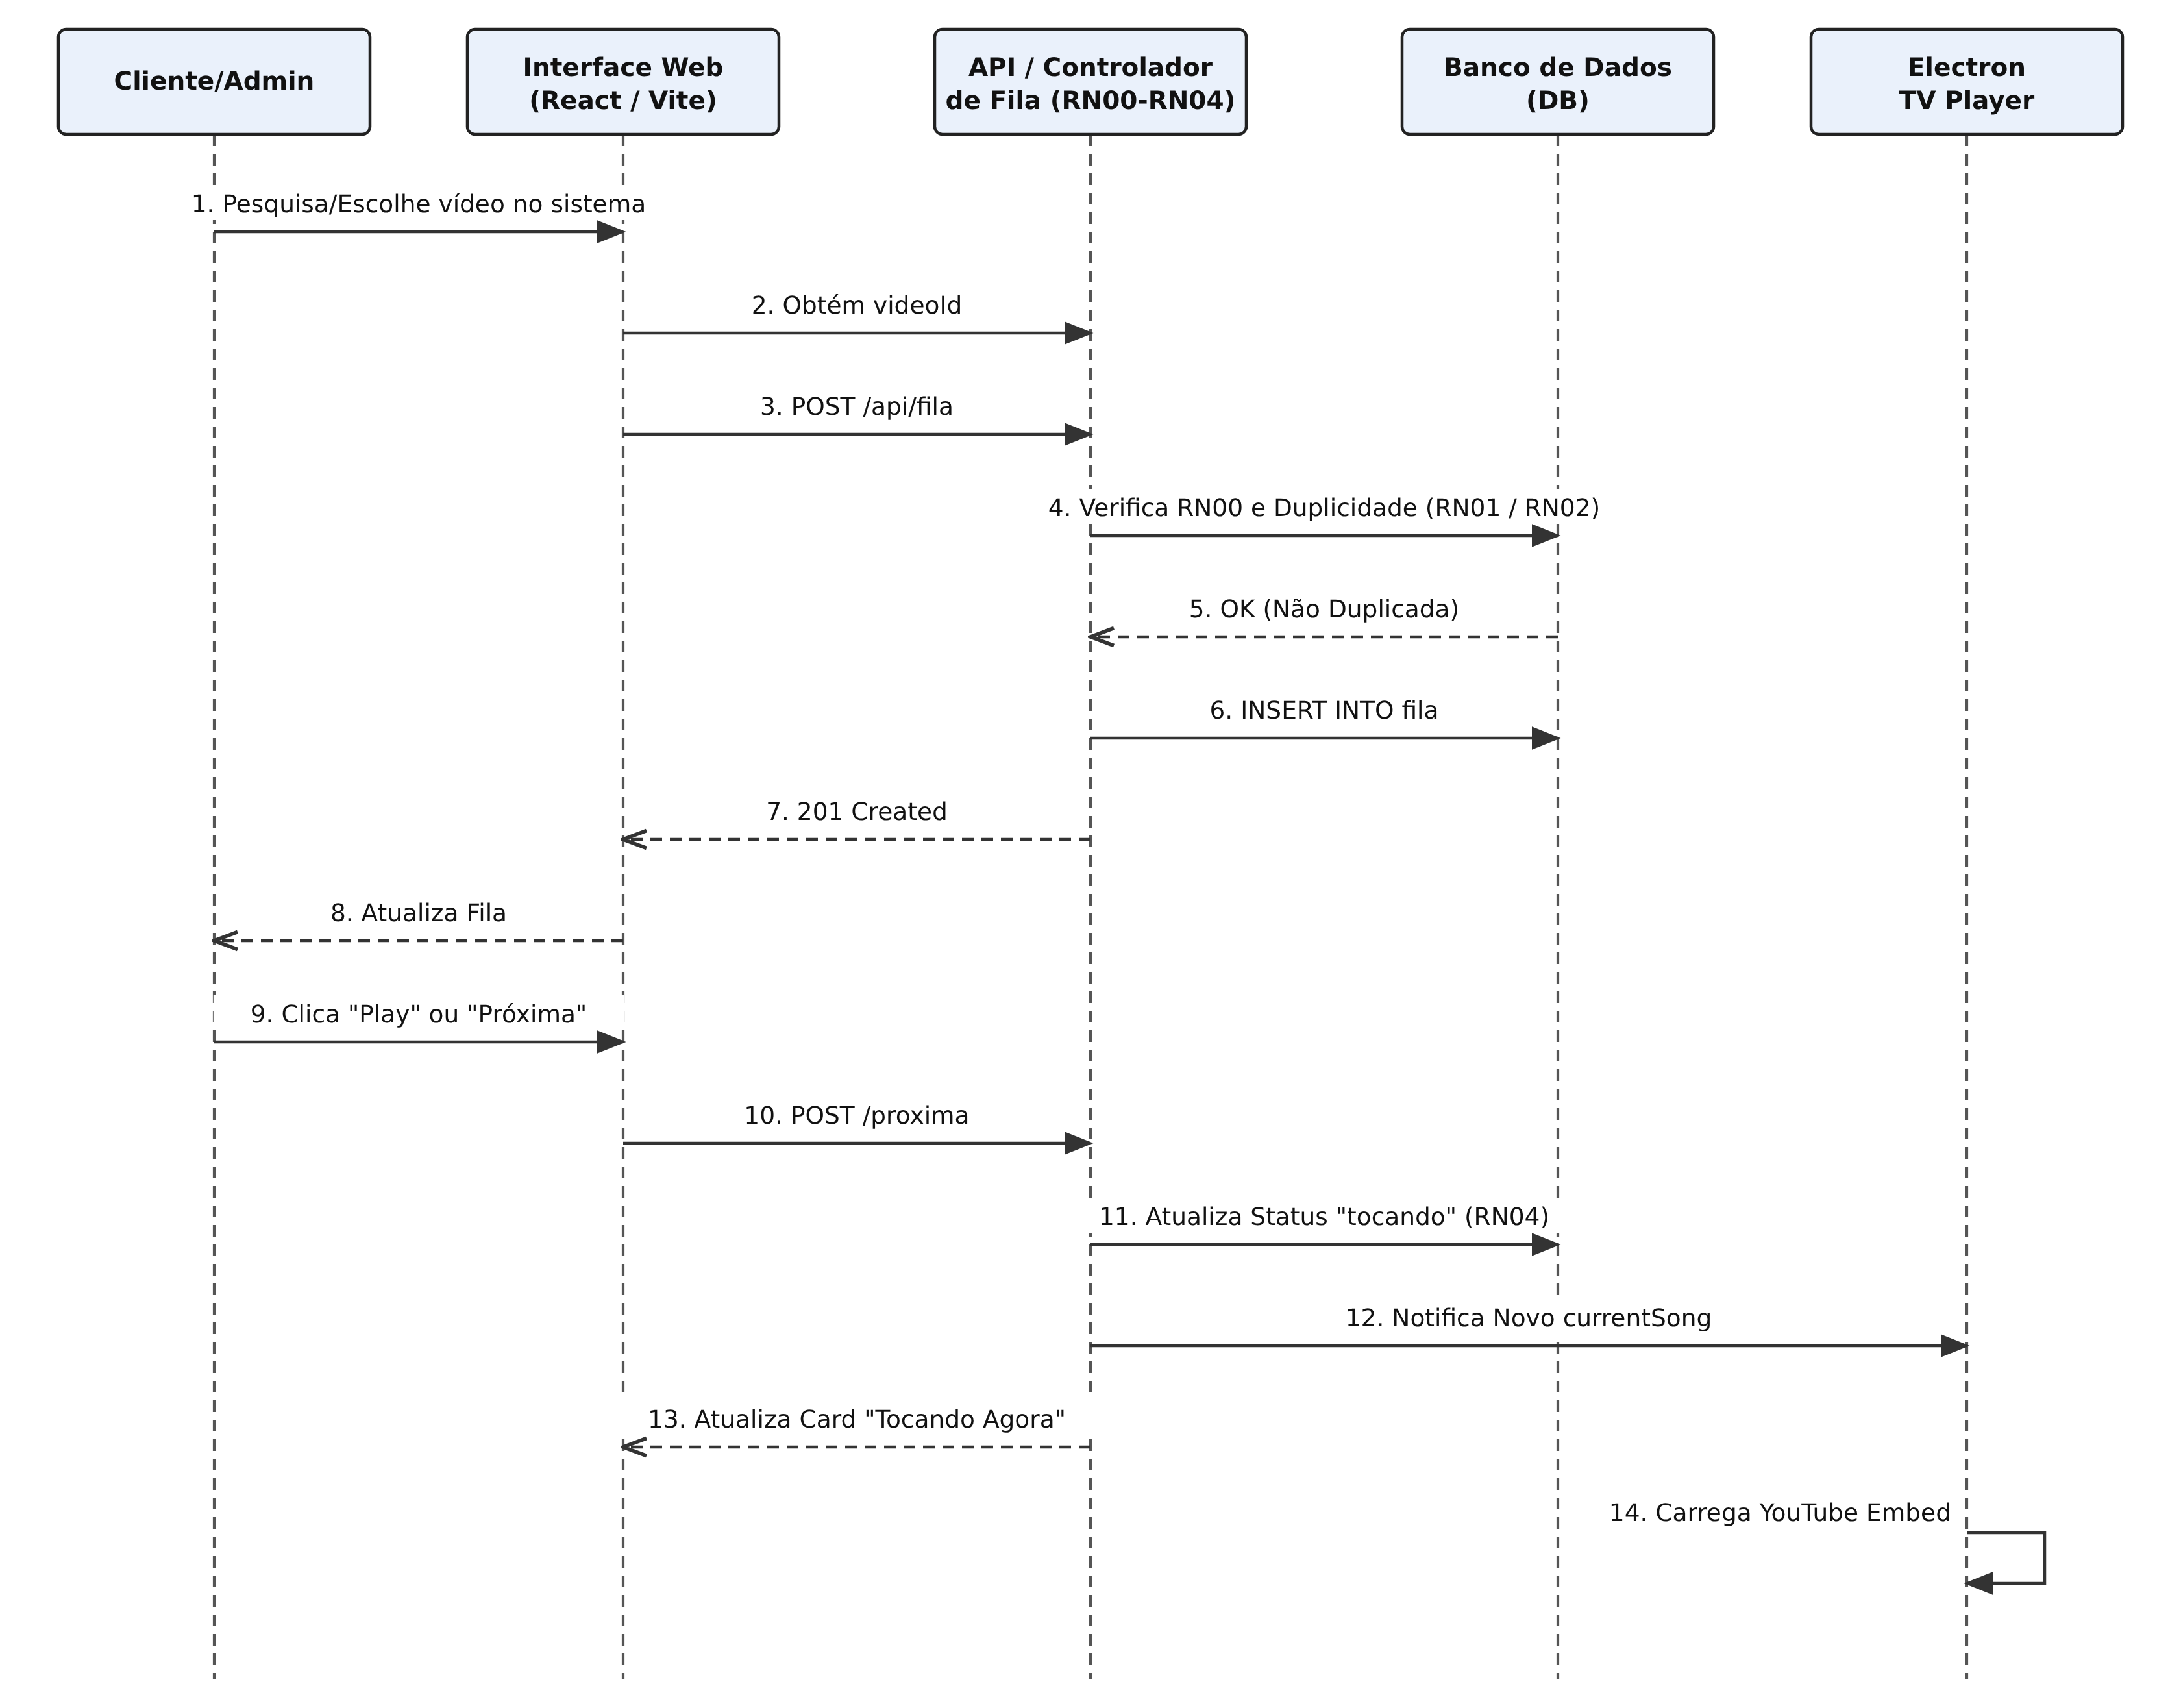
\includegraphics[width=\textwidth,height=0.78\textheight,keepaspectratio]{imagens/diagrama_sequencia.png}
\end{center}
\legend{Fonte: Elaborado pelos autores (2026).}
\end{caixa}

\section{Tecnologias Utilizadas}

A seleção tecnológica do projeto priorizou ferramentas modernas, multiplataforma e amplamente adotadas pelo mercado de desenvolvimento de software, consolidadas na Tabela \ref{tab:tecnologias}.

\begin{table}[H]
\IBGEtab{%
  \caption{Tecnologias, frameworks e ferramentas utilizadas no projeto.}%
  \label{tab:tecnologias}%
}{%
  \footnotesize
  \begin{tabularx}{\textwidth}{p{3.2cm}p{3.4cm}X}
    \toprule
    \textbf{Categoria} & \textbf{Tecnologia / Ferramenta} & \textbf{Função Desempenhada no Projeto} \\
    \midrule
    Front-end Web & React 19 + Vite \cite{react2025} & Construção reativa da interface de controle e fila (\textit{Single Page Application}), com atualização instantânea de estado e empacotamento rápido via Vite. \\
    \addlinespace
    Aplicação Desktop (Telão) & Electron \cite{electron2025} & Encapsulamento nativo do reprodutor \textit{Karaokê TV Player}, garantindo execução dedicada em tela cheia, controle de políticas de rede e isolamento de contexto. \\
    \addlinespace
    Back-end / API Orquestradora & Java 21 & Desenvolvimento da API RESTful centralizada, aplicação das regras de negócio (RN00--RN04), autenticação e orquestração da fila de reprodução. \\
    \addlinespace
    Banco de Dados & MySQL & Sistema de Gerenciamento de Banco de Dados relacional utilizado para a persistência estruturada das tabelas \texttt{usuario}, \texttt{musica}, \texttt{letra} e \texttt{fila} conforme modelado no arquivo \texttt{Conceitual.brM3}. \\
    \addlinespace
    Modelagem de Engenharia & brModelo, UMLet (\texttt{.uxf}) e Draw.io & Construção do Modelo Entidade-Relacionamento conceitual e dos diagramas arquiteturais e UML do sistema. \\
    \addlinespace
    Versionamento de Código & Git e GitHub & Controle de versão distribuído e colaboração entre os integrantes da equipe no repositório do projeto (\texttt{MurilloAssis/Projeto-Extensao-Karaoke}). \\
    \addlinespace
    Gestão e Documentação & Trello e \LaTeX\ / Overleaf & Acompanhamento das tarefas ágeis em quadro Kanban e editoração científica do relatório segundo as normas da ABNT. \\
    \bottomrule
  \end{tabularx}%
}{%
  \fonte{Elaborado pelos autores (2026).}%
}
\end{table}

\section{Segurança e Controle de Acesso}

O projeto de segurança e controle de acesso do sistema contempla quatro camadas de proteção, alinhadas às boas práticas de desenvolvimento seguro e à Lei Geral de Proteção de Dados Pessoais -- LGPD (Lei n{\textordmasculine} 13.709/2018) \cite{brasil2018lgpd}:

\begin{enumerate}
  \item \textbf{Autenticação e Controle de Acesso Baseado em Papéis (RBAC):} distinção entre sessões de \texttt{cliente} (autorizadas apenas a consultar o catálogo/fila e submeter pedidos sob as regras RN00--RN02) e sessões de \texttt{admin} (autorizadas a controlar a reprodução do palco conforme a RN03), utilizando senhas com hash \texttt{bcrypt} e tokens JWT;
  \item \textbf{Segurança no Processo Electron (\textit{Context Isolation} e CSP):} configuração da janela do \textit{Karaokê TV Player} com \texttt{contextIsolation: true}, \texttt{nodeIntegration: false} e diretivas estritas de \textit{Content Security Policy} (CSP) que limitam a origem de scripts e quadros (\texttt{frame-src}) exclusivamente à aplicação local e ao domínio oficial de incorporação do YouTube;
  \item \textbf{Isolamento de Variáveis de Ambiente e Credenciais de Banco:} armazenamento das credenciais de conexão ao MySQL e chaves de assinatura em variáveis de ambiente isoladas do código-fonte via \texttt{.gitignore};
  \item \textbf{Minimização de Dados (Art. 6{\textordmasculine} da LGPD):} coleta restrita ao nome de chamada ao palco e e-mail de identificação do participante.
\end{enumerate}

O Quadro \ref{quad:estados} apresenta o \textbf{Diagrama de Estados UML} que formaliza as transições de estado permitidas para um pedido musical dentro da fila (RN04) e as guardas de autorização (RN03) exigidas em cada transição.

\Needspace{20cm}
\begin{caixa}{Diagrama de Estados UML -- Ciclo de Vida de um Pedido Musical na Fila (RN03 e RN04)}{quad:estados}
\begin{center}
  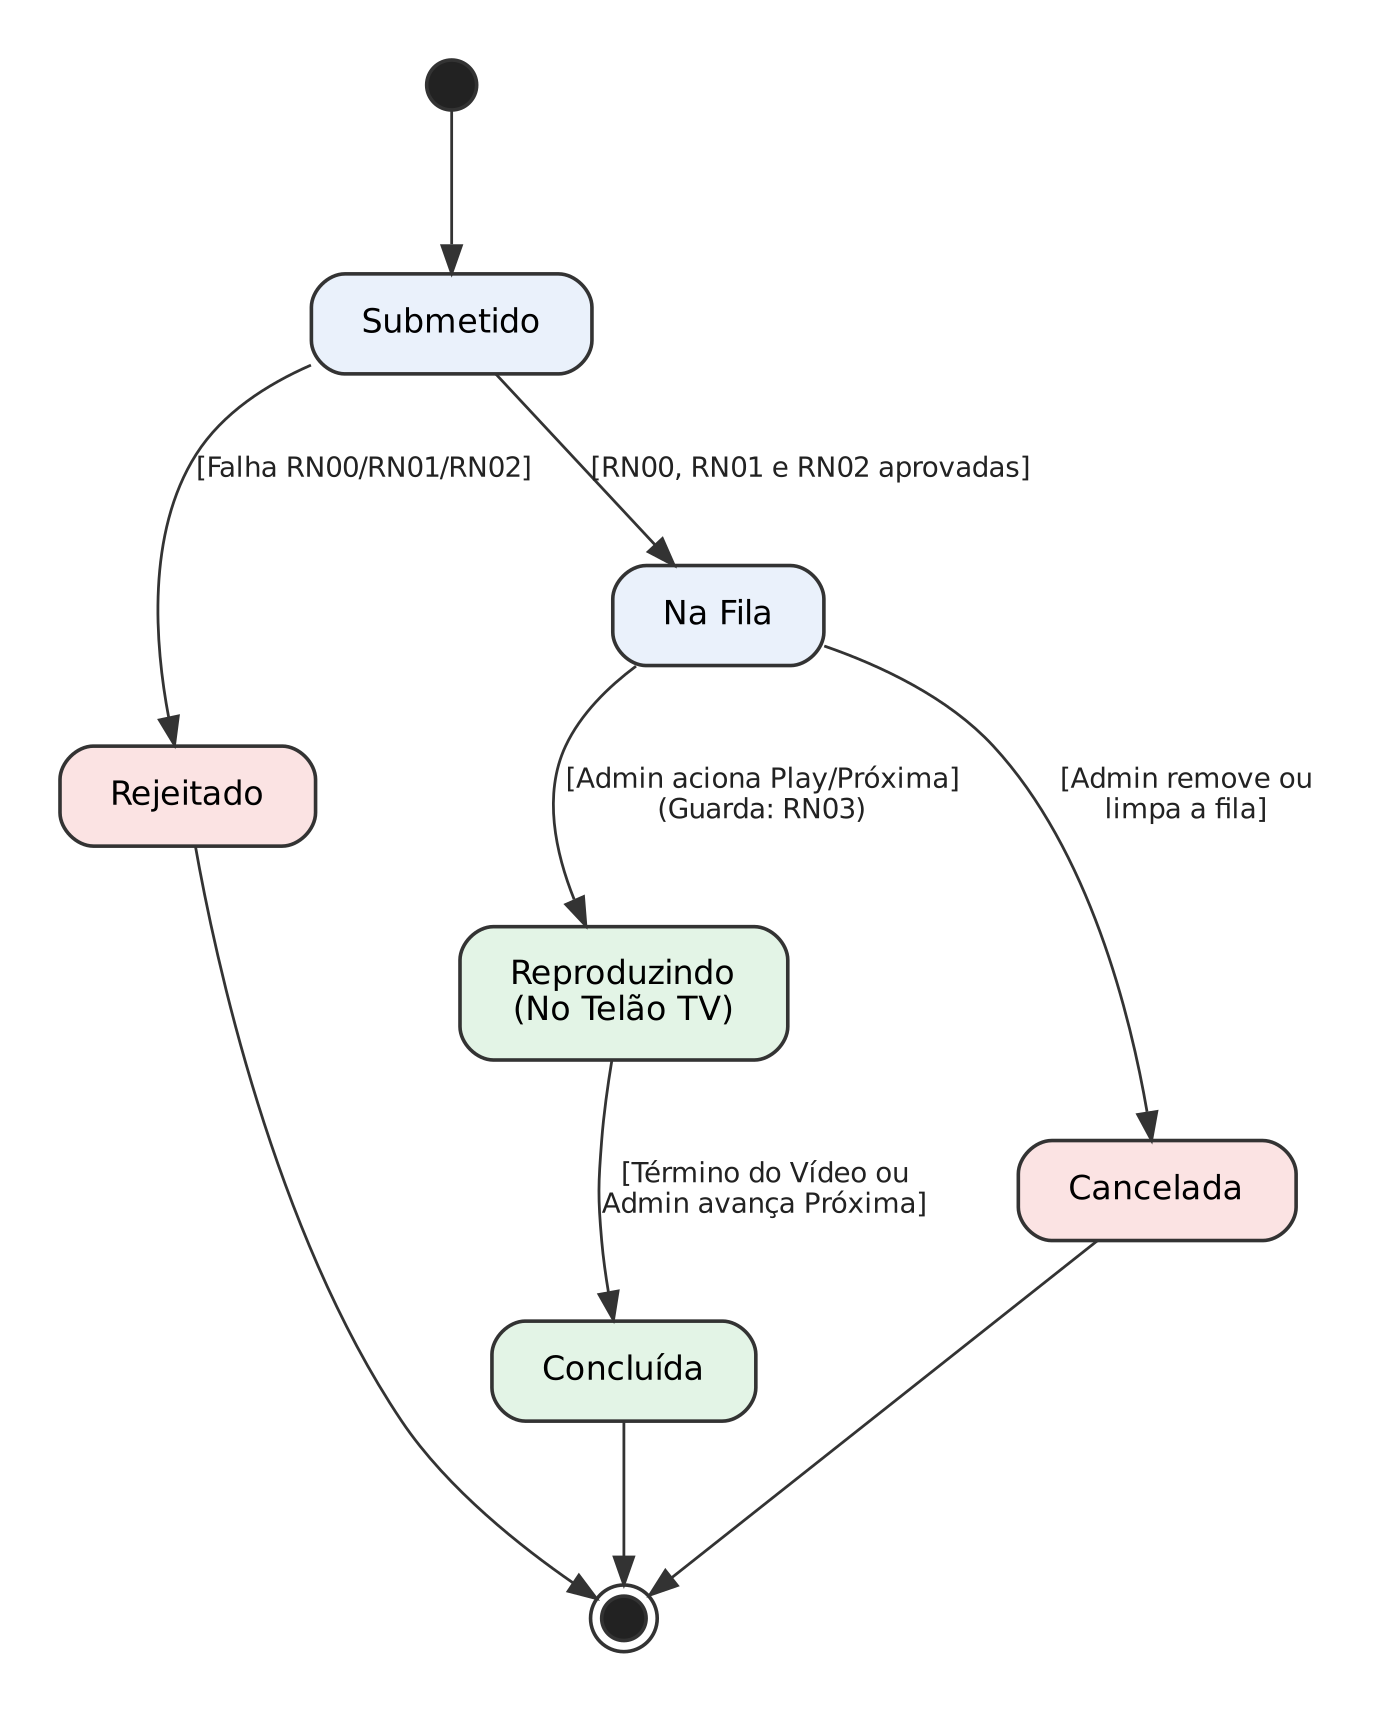
\includegraphics[width=\textwidth,height=0.78\textheight,keepaspectratio]{imagens/diagrama_estados.png}
\end{center}
\legend{Fonte: Elaborado pelos autores (2026).}
\end{caixa}

%% -------------------------------------------------------------------------- %%

\chapter{Implementação} \label{cap:implementacao}

Este capítulo descreve a materialização do projeto \textbf{Karaokê Apache} em software. Considerando que o projeto encontra-se atualmente em \textbf{fase de Produto Mínimo Viável (MVP)}, as seções a seguir documentam o ambiente configurado, a estrutura da aplicação, os componentes já implementados e validados no núcleo funcional da Prova de Conceito (PoC/MVP), a integração entre a fila web e o reprodutor Electron, bem como os testes preliminares, resultados parciais e limitações próprias do estágio atual de desenvolvimento.

\section{Ambiente de Desenvolvimento}

O desenvolvimento e a execução do MVP foram conduzidos utilizando um ambiente padronizado entre os integrantes da equipe de desenvolvimento, composto pelos seguintes recursos de hardware, sistema operacional e ferramentas:

\begin{itemize}
  \item \textbf{Estações de Trabalho e Sistemas Operacionais:} computadores pessoais dos desenvolvedores e máquinas dos laboratórios de informática do IFSP -- Campus São Paulo, executando sistemas operacionais Windows 10/11 (64 bits) e distribuições Linux;
  \item \textbf{Linguagens, Banco de Dados e Ferramentas de Construção:} kit de desenvolvimento \textit{Java 21 (JDK 21)} para a API de back-end, Sistema de Gerenciamento de Banco de Dados \textit{MySQL}, ambiente \textit{Node.js} (com gerenciador de pacotes \texttt{npm}), empacotador \textit{Vite} e framework \textit{Electron} para o front-end e reprodutor de telão;
  \item \textbf{IDEs e Repositório de Código no GitHub:} desenvolvimento utilizando \textit{Visual Studio Code} / IDEs Java e versionamento distribuído centralizado no repositório oficial \url{https://github.com/MurilloAssis/Projeto-Extensao-Karaoke}.
\end{itemize}

\section{Estrutura da Aplicação}

A organização física de diretórios e pacotes da aplicação no estágio atual de MVP separa claramente o código do processo nativo do Electron, os componentes visuais em React e a camada de serviços/estado da fila. O Quadro \ref{quad:pacotes} apresenta o \textbf{Diagrama de Pacotes UML} da estrutura implementada.

\Needspace{11.2cm}
\begin{caixa}{Diagrama de Pacotes UML -- Estrutura de Diretórios e Módulos do MVP}{quad:pacotes}
\begin{center}
  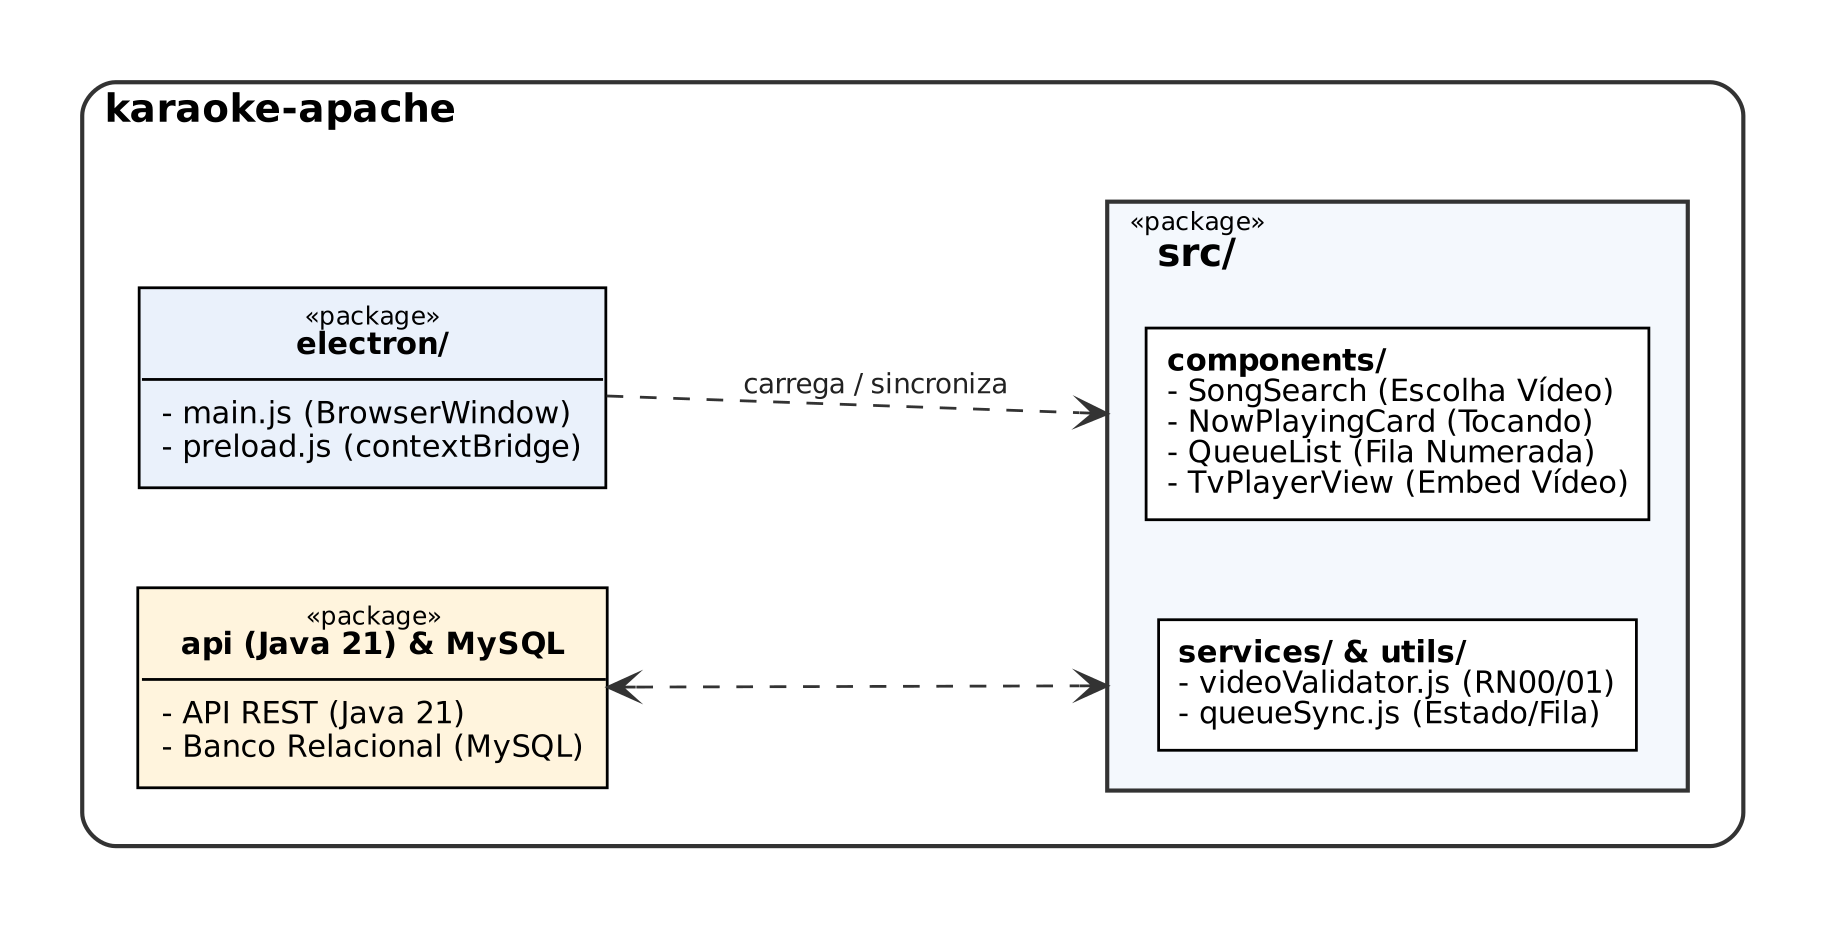
\includegraphics[width=\textwidth,height=0.78\textheight,keepaspectratio]{imagens/diagrama_pacotes.png}
\end{center}
\legend{Fonte: Elaborado pelos autores (2026).}
\end{caixa}

\section{Implementação dos Componentes}

Na fase atual de MVP, a implementação priorizou os componentes críticos responsáveis por validar a proposta central do sistema: receber pedidos musicais, organizar a fila sem duplicidades e controlar remotamente o que é reproduzido na TV do bar.

\begin{itemize}
  \item \textbf{Componente \textit{Pedido de Música}:} foi construído o módulo que permite a seleção de vídeos de karaokê pelo sistema e valida o identificador do vídeo escolhido. Caso o vídeo seja inválido/indisponível (RN00) ou o identificador já conste na fila ativa ou em reprodução (RN01), a inclusão na fila é bloqueada;
  \item \textbf{Componente \textit{Fila}:} foi implementada a gestão reativa da lista de músicas (\texttt{queue}) e da faixa ativa (\texttt{currentSong}). A interface permite adicionar itens ao final da fila, acionar o botão \textbf{Play} em qualquer posição, avançar para a \textbf{Próxima música} (promovendo automaticamente o primeiro item da fila para reprodução), excluir itens individuais e limpar toda a fila;
  \item \textbf{Componente \textit{Reprodutor} -- \textit{Karaokê TV Player}:} foi implementado o processo principal do Electron (\texttt{main.js}) que instancia uma janela dedicada (\texttt{BrowserWindow}) conectada ao estado da fila. Sempre que o estado de \texttt{currentSong} é atualizado na interface de controle, o \textit{Karaokê TV Player} exibe o código da faixa no cabeçalho (\textit{``Conectado -- Tocando: [ID]''}) e renderiza o player de vídeo do YouTube;
  \item \textbf{Componente \textit{Usuários} e Persistência Relacional (Java 21 e MySQL):} compreende a estruturação da API em Java 21 integrada ao banco de dados MySQL (\texttt{Conceitual.brM3}) para gerenciamento das entidades \texttt{usuario} (\texttt{admin}/\texttt{cliente}), \texttt{musica}, \texttt{letra} e \texttt{fila}.
\end{itemize}

\section{Integração dos Módulos}

Em ambiente de execução, os módulos da aplicação comunicam-se na mesma rede local do estabelecimento: o servidor web disponibiliza a interface de controle e fila em React/Vite (\texttt{http://localhost:5173}), enquanto a instância do aplicativo desktop \textbf{Karaokê TV Player} em Electron permanece aberta na saída de vídeo secundária conectada ao telão do palco. Qualquer ação de adição ou troca de música efetuada no controlador web propaga-se instantaneamente para a janela do Electron. O Quadro \ref{quad:implantacao} apresenta o \textbf{Diagrama de Implantação UML} que ilustra a topologia física de execução da solução no Apache Gru Rock Bar.

\Needspace{7.9cm}
\begin{caixa}{Diagrama de Implantação UML -- Topologia de Execução no Apache Gru Rock Bar}{quad:implantacao}
\begin{center}
  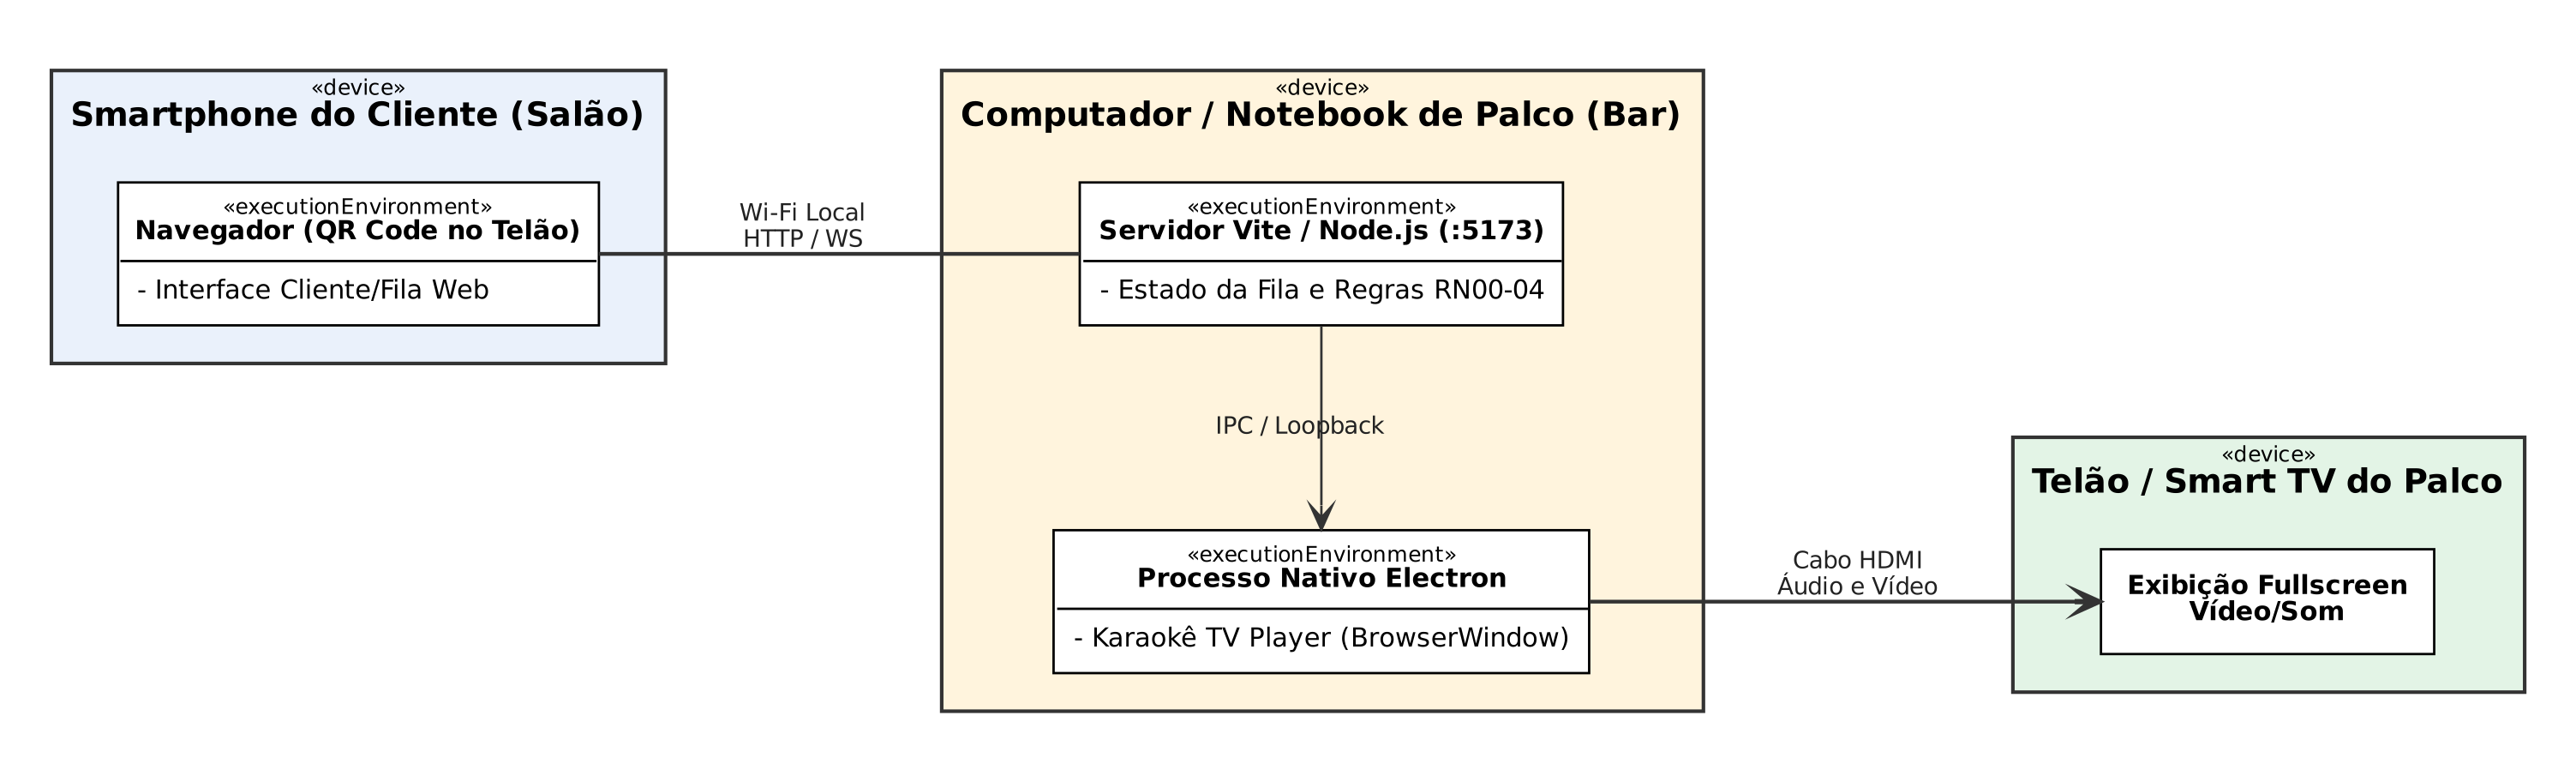
\includegraphics[width=\textwidth,height=0.78\textheight,keepaspectratio]{imagens/diagrama_implantacao.png}
\end{center}
\legend{Fonte: Elaborado pelos autores (2026).}
\end{caixa}

\section{Testes Realizados}

Como o projeto encontra-se em estágio de MVP, os procedimentos de teste concentraram-se na validação prática dos fluxos essenciais implementados na Prova de Conceito (registrada no vídeo \texttt{Poc.mp4}) e na verificação do funcionamento do reprodutor Electron em diferentes ambientes de rede. A Tabela \ref{tab:testes_mvp} sumariza os testes realizados até o momento.

\begin{table}[H]
\IBGEtab{%
  \caption{Testes preliminares realizados sobre a Prova de Conceito e o MVP.}%
  \label{tab:testes_mvp}%
}{%
  \footnotesize
  \begin{tabularx}{\textwidth}{p{1.3cm}p{3.2cm}X p{2.2cm}}
    \toprule
    \textbf{ID} & \textbf{Aspecto Avaliado} & \textbf{Procedimento Executado e Resultado Observado} & \textbf{Situação no MVP} \\
    \midrule
    TST-01 & Escolha e Adição de Vídeo à Fila pelo Sistema & Seleção de vídeos de karaokê (como \textit{Still Loving You -- Scorpions}, ID \texttt{R2F\_hGwD26g}, e \textit{Oh! Darling -- The Beatles}) na interface web; os itens foram validados e listados corretamente na fila numerada. & Validado (\texttt{Poc.mp4}) \\
    \addlinespace
    TST-02 & Sincronização do Comando \textit{Play} com o Electron & Acionamento do botão \textit{Play} na interface web (\texttt{localhost:5173}); o \textit{Karaokê TV Player} em Electron atualizou imediatamente o status para \textit{Conectado -- Tocando} e iniciou o vídeo. & Validado (\texttt{Poc.mp4}) \\
    \addlinespace
    TST-03 & Avanço de Faixa (\textit{Próxima música}) e Limpeza & Acionamento do botão \textit{Próxima música} e exclusão de itens; a fila avançou corretamente na ordem FIFO e atualizou a tela do reprodutor. & Validado (\texttt{Poc.mp4}) \\
    \addlinespace
    TST-04 & Bloqueio de Música Duplicada na Fila (RN01) & Tentativa de inserção repetida de um vídeo já presente na fila ativa; o sistema bloqueou a duplicidade e preservou a integridade da fila. & Validado \\
    \addlinespace
    TST-05 & Integração da API Java 21 com o MySQL & Testes de persistência das entidades modeladas e autenticação por perfil (\texttt{admin}/\texttt{cliente}) no banco de dados MySQL. & Em andamento (MVP) \\
    \bottomrule
  \end{tabularx}%
}{%
  \fonte{Elaborado pelos autores (2026).}%
}
\end{table}

\section{Resultados Obtidos}

Até o presente estágio de MVP, os resultados alcançados confirmam a viabilidade técnica da arquitetura proposta e atendem ao propósito central que motivou o projeto junto ao Apache Gru Rock Bar:

\begin{itemize}
  \item \textbf{Validação prática da orquestração entre Web e Electron (\texttt{Poc.mp4}):} comprovou-se que o operador do bar pode gerenciar a fila de músicas em uma interface web limpa enquanto o aplicativo desktop \textbf{Karaokê TV Player} reproduz automaticamente os vídeos selecionados em uma janela independente dedicada à TV, eliminando a necessidade de procurar vídeos manualmente e arrastar abas para o telão;
  \item \textbf{Consolidação da arquitetura e das regras do negócio:} o levantamento junto ao parceiro resultou em um conjunto coerente de regras de negócio (RN00 a RN04), modelo de dados (\texttt{Conceitual.brM3}) e divisão modular em quatro componentes (\textit{Usuários}, \textit{Fila}, \textit{Pedido de Música} e \textit{Reprodutor});
  \item \textbf{Adequação econômica ao parceiro:} toda a pilha tecnológica validada no MVP opera com custo zero de licenciamento, podendo ser executada diretamente no equipamento já disponível no estabelecimento.
\end{itemize}

\section{Limitações da Implementação}

Por tratar-se de uma versão em fase de Produto Mínimo Viável (MVP), registram-se as seguintes limitações atuais e pontos conhecidos que orientam a continuidade imediata do desenvolvimento:

\begin{itemize}
  \item \textbf{Escopo parcial da persistência e autenticação na PoC inicial:} no recorte validado na PoC (\texttt{Poc.mp4}), a fila e o estado da música atual operam de forma reativa em sessão local para validar a comunicação com o Electron, estando o acoplamento completo das telas de login/cadastro com o banco de dados relacional em fase de finalização no MVP;
  \item \textbf{Restrições externas de incorporação (\textit{embed}) do YouTube:} alguns vídeos musicais específicos possuem bloqueio de reprodução em quadros externos definido pelos canais proprietários no YouTube; no estágio atual do MVP, caso um link com bloqueio seja inserido, o operador utiliza o botão \textit{Próxima música} para avançar imediatamente para a faixa seguinte;
  \item \textbf{Transição automática ao final do vídeo:} na versão inicial do protótipo, o avanço para a próxima música pode ser acionado manualmente pelo organizador no botão \textit{Próxima música} ao término dos aplausos no palco, prevendo-se o gatilho opcional de avanço automático via eventos da API de IFrame do YouTube (\texttt{onStateChange}) nos incrementos seguintes.
\end{itemize}

%% -------------------------------------------------------------------------- %%

\chapter{Conclusão} \label{cap:conclusao}

Este capítulo encerra o documento sintetizando as considerações finais sobre o desenvolvimento do projeto \textbf{Karaokê Apache} até a sua fase atual de MVP, relatando as principais dificuldades superadas pela equipe e apresentando as possibilidades de evolução futura do sistema.

\section{Considerações Finais}

O desenvolvimento do projeto \textbf{Karaokê Apache} demonstrou como a aplicação estruturada de conceitos de Engenharia de Software, Análise de Sistemas e Arquitetura de Aplicações Distribuídas permite construir uma solução tecnológica diretamente alinhada à realidade de um pequeno negócio local. Ao investigar a rotina da \textit{Noite de Karaokê} no estabelecimento parceiro \textbf{Apache Gru Rock Bar}, em Guarulhos -- SP, foi possível traduzir gargalos operacionais concretos -- antes resolvidos no improviso com anotações em papel e janelas manuais de navegador -- em requisitos objetivos, regras de negócio bem definidas (RN00 a RN04) e uma arquitetura modular clara.

Mesmo encontrando-se em fase de Produto Mínimo Viável (MVP), os resultados obtidos na implementação da Prova de Conceito (\texttt{Poc.mp4}) cumpriram o objetivo de validar o núcleo mais sensível da solução: a sincronização em tempo real entre a fila web em React/Vite e o reprodutor desktop dedicado \textbf{Karaokê TV Player} em Electron. Dessa forma, o projeto entrega ao estabelecimento parceiro uma base funcional sólida, gratuita e adaptada à sua infraestrutura física, ao mesmo tempo em que consolida a formação prática dos estudantes do IFSP.

\section{Dificuldades Encontradas}

Ao longo do ciclo de levantamento, modelagem e implementação do MVP, a equipe enfrentou e solucionou três dificuldades principais:

\begin{enumerate}
  \item \textbf{Sincronização em tempo real entre a fila web e o reprodutor desktop:} garantir que as ações de controle da fila refletissem imediatamente na janela dedicada do \textit{Karaokê TV Player} em Electron sem necessidade de recarregar a página exigiu o desacoplamento claro entre o estado da fila e o componente de exibição;
  \item \textbf{Políticas de incorporação (\textit{embed}) e \textit{autoplay} de vídeos:} navegadores modernos e o próprio YouTube impõem restrições a vídeos embarcados e ao início automático de áudio, o que exigiu testes específicos dentro do container Chromium do Electron e a inclusão de controles diretos (\textit{Play} e \textit{Próxima música}) para o operador do palco;
  \item \textbf{Calibragem do escopo para o calendário semestral:} foi necessário delimitar criteriosamente o escopo do MVP, descartando ideias iniciais que criariam barreiras de uso para os clientes do bar (como obrigar o download de um aplicativo nativo nas lojas móveis) em favor de uma interface web acessível instantaneamente via QR Code no telão.
\end{enumerate}

\section{Trabalhos Futuros}

Como continuidade natural após a conclusão e implantação definitiva do MVP no Apache Gru Rock Bar, destacam-se os seguintes trabalhos futuros:

\begin{itemize}
  \item \textbf{Implementação do módulo de letras no celular e painel de estatísticas musicais:} ativar na próxima etapa do projeto o preenchimento e exibição da tabela \texttt{letra} (já estruturada na modelagem de dados) para acompanhamento no celular, bem como relatórios das músicas mais cantadas no Apache Gru Rock Bar;
  \item \textbf{Notificação automática de proximidade na fila:} emitir um alerta visual no celular do cliente quando faltar apenas uma música para sua chamada ao palco;
  \item \textbf{Detecção automática de bloqueio de \textit{embed} via YouTube IFrame API:} validar preventivamente no momento do pedido se o vídeo do YouTube permite reprodução embarcada, sugerindo automaticamente versões alternativas de karaokê;
  \item \textbf{Interação da plateia e integração com o cardápio digital da casa:} permitir que as mesas enviem reações visuais para o telão durante as apresentações e disponibilizar um atalho rápido na tela da fila para o cardápio de bebidas e porções do bar.
\end{itemize}



%% Finalizações para o PDF
\bookmarksetup{startatroot}

%% Elementos pós-textuais: Referências, Apêndices, Anexos, etc.
% !TEX root = ../documento.tex
%% %%%%%%%%%%%%%%%%%%%%%%%%%%%%%%%%%%%%%%%%% %%
%% Elementos Pós Textuais
%% ----------------------
%% 
%% Segundo o manual do IFPI, eles devem ser os seguintes (nessa ordem):
%% 1. Referências (obrigatório)
%% 2. Glossário (opcional)
%% 3. Apêndice (opcional)
%% 4. Anexos (opcional)
%% 5. Índices (opcional)
%% %%%%%%%%%%%%%%%%%%%%%%%%%%%%%%%%%%%%%%%%% %%

%% Indica ao LaTeX que a partir deste ponto ficarão os elementos pós-textuais
\postextual

%% 01: Referências bibliográficas
%% Referências bibliográficas

\bibliography{bibliografia}

%% 02: Glossário
%% Glossário
%\glossary

%% 03: Apêndices
\begin{apendicesenv}

\apendiceitem{Especificação XML do Diagrama de Componentes no UMLet}{apendice:uml}

O trecho XML reproduzido na Listagem \ref{lst:umlet} corresponde ao arquivo \texttt{diagrama\_de\_componentes.uxf}, produzido pelos autores na ferramenta UMLet para modelar os componentes \textit{Usuários}, \textit{Fila}, \textit{Pedido de Música} e \textit{Reprodutor}.

\begin{lstlisting}[language=XML, caption={Estrutura do arquivo diagrama\_de\_componentes.uxf (UMLet).}, label={lst:umlet}]
<?xml version="1.0" encoding="UTF-8" standalone="no"?>
<diagram program="umlet" version="15.1">
  <zoom_level>10</zoom_level>
  <element>
    <id>UMLGeneric</id>
    <coordinates><x>250</x><y>80</y><w>430</w><h>110</h></coordinates>
    <panel_attributes>symbol=component
Usuarios</panel_attributes>
  </element>
  <element>
    <id>UMLGeneric</id>
    <coordinates><x>250</x><y>280</y><w>430</w><h>100</h></coordinates>
    <panel_attributes>symbol=component
Fila</panel_attributes>
  </element>
  <element>
    <id>UMLGeneric</id>
    <coordinates><x>160</x><y>530</y><w>200</w><h>100</h></coordinates>
    <panel_attributes>symbol=component
Pedido de Musica</panel_attributes>
  </element>
  <element>
    <id>UMLGeneric</id>
    <coordinates><x>520</x><y>520</y><w>200</w><h>100</h></coordinates>
    <panel_attributes>symbol=component
Reprodutor</panel_attributes>
  </element>
</diagram>
\end{lstlisting}

\apendiceitem{Trechos de Código-Fonte do MVP (Electron e Validação da Fila)}{apendice:codigo}

A Listagem \ref{lst:electron_main} apresenta o script principal de inicialização do \textbf{Karaokê TV Player} em Electron (\texttt{main.js}), incluindo a configuração da janela dedicada de exibição e o isolamento de contexto.

\begin{lstlisting}[language=Java, caption={Inicialização do reprodutor desktop Karaokê TV Player em Electron (main.js).}, label={lst:electron_main}]
const { app, BrowserWindow } = require('electron');
const path = require('path');

function createPlayerWindow() {
  const playerWindow = new BrowserWindow({
    width: 1280,
    height: 720,
    title: 'Karaoke TV Player - Apache Gru Rock Bar',
    autoHideMenuBar: true,
    webPreferences: {
      preload: path.join(__dirname, 'preload.js'),
      contextIsolation: true,
      nodeIntegration: false,
      sandbox: true
    }
  });

  const playerUrl = process.env.ELEC_PLAYER_URL || 'http://localhost:5173/player';
  playerWindow.loadURL(playerUrl);
}

app.whenReady().then(() => {
  createPlayerWindow();
});
\end{lstlisting}

A Listagem \ref{lst:youtube_parser} demonstra a função de extração de identificadores de vídeo do YouTube e validação das regras RN00 e RN01 antes da inserção na fila.

\begin{lstlisting}[language=Java, caption={Extração de ID do YouTube e validação anti-duplicidade na fila (RN00 e RN01).}, label={lst:youtube_parser}]
export function extractYouTubeId(url) {
  if (!url || typeof url !== 'string') return null;
  const regex = /(?:youtube\.com\/(?:[^\/]+\/.+\/|(?:v|e(?:mbed)?)\/|.*[?&]v=)|youtu\.be\/)([^"&?\/\s]{11})/i;
  const match = url.trim().match(regex);
  return match ? match[1] : null;
}

export function validateQueueInsertion(videoUrl, customTitle, activeQueue, currentSong) {
  const videoId = extractYouTubeId(videoUrl);
  if (!videoId) {
    return { valid: false, error: 'RN00: Link do YouTube invalido ou nao suportado.' };
  }
  const alreadyPlaying = currentSong && currentSong.videoId === videoId;
  const alreadyInQueue = activeQueue.some((item) => item.videoId === videoId);
  if (alreadyPlaying || alreadyInQueue) {
    return { valid: false, error: 'RN01: Esta musica ja esta na fila ou em reproducao.' };
  }
  return {
    valid: true,
    songItem: {
      videoId,
      title: customTitle?.trim() || `Musica (${videoId})`,
      status: 'na_fila',
      requestedAt: new Date().toISOString()
    }
  };
}
\end{lstlisting}

\end{apendicesenv}

%% -------------------------------------------------------------------------- %%


%% 04: Anexos
\begin{anexosenv}

\anexoitem{Referência Normativa -- Art. 6{\textordmasculine} da Lei Geral de Proteção de Dados Pessoais (Lei n{\textordmasculine} 13.709/2018)}{anexo:lgpd}

Transcrição do Art. 6{\textordmasculine} da Lei n{\textordmasculine} 13.709, de 14 de agosto de 2018 (LGPD) \cite{brasil2018lgpd}, utilizado como referência normativa para as restrições de privacidade e minimização de dados cadastrais no sistema \textbf{Karaokê Apache}:

\begin{citacao}
Art. 6{\textordmasculine} As atividades de tratamento de dados pessoais deverão observar a boa-fé e os seguintes princípios:

I -- finalidade: realização do tratamento para propósitos legítimos, específicos, explícitos e informados ao titular, sem possibilidade de tratamento posterior de forma incompatível com essas finalidades;

II -- adequação: compatibilidade do tratamento com as finalidades informadas ao titular, de acordo com o contexto do tratamento;

III -- necessidade: limitação do tratamento ao mínimo necessário para a realização de suas finalidades, com abrangência dos dados pertinentes, proporcionais e não excessivos em relação às finalidades do tratamento de dados;

VII -- segurança: utilização de medidas técnicas e administrativas aptas a proteger os dados pessoais de acessos não autorizados e de situações acidentais ou ilícitas de destruição, perda, alteração, comunicação ou difusão.
\end{citacao}

\end{anexosenv}


%% 05: Índices
%% Índices
%\phantompart \printindex

%% Capa do CD (opcional)
%%% Isso aqui cria a capa do CD, no final do documento :)
\newpage
\thispagestyle{empty}
\begin{center}
\covers[{\vspace{1.5cm} \Large \MakeUppercase{Curso de \imprimirnomedocurso} \\ \vspace{1cm} \textbf{\imprimirautor} \\ \vspace{0.5cm} {TÍTULO: \imprimirtitulo}}]{
	{\vspace{1.5cm} \MakeUppercase{Curso de \imprimirnomedocurso} \\ \vspace{1cm} {\textbf{\imprimirautor}} \\ \vspace{0.3cm} {TÍTULO: \imprimirtitulo} \\ \vspace{1.5cm} \MakeUppercase{\imprimirlocal} \par \imprimirdata}
}{
	\MakeUppercase{\tiny \imprimirtitulo}
}
\end{center}

\end{document}
